% ============================================================================
% CausalBKMR: Causal Inference for Health Effects of Time-varying Correlated
% Environmental Mixtures
%
% Full manuscript for Nature Methods, using Springer Nature LaTeX template.
%
% IMPORTANT: This file expects sn-jnl.cls and the sn-nature bibliography
% style. These are NOT on CTAN. To compile:
%   (1) In Overleaf: import the Springer Nature LaTeX template
%       https://www.overleaf.com/latex/templates/springer-nature-latex-template/myxmhdsbzkyd
%       Copy sn-jnl.cls and sn-nature.bst into this project.
%   (2) Locally: download the template zip from Springer Nature and place
%       sn-jnl.cls in the repo root (do not commit if license-restricted).
%
% This file stitches together the modular sections in sections/ via \input{}.
% Each section file is plain content (no preamble), so Application.tex and
% Supplementary.tex can reuse the same .tex sources.
% ============================================================================

\documentclass[sn-nature]{sn-jnl}

% Additional packages needed by our content (tikz for DAG, subcaption for side-by-side figures)
\usepackage{tikz}
\usetikzlibrary{arrows.meta, positioning, bending}
\usepackage{subcaption}
\usepackage{graphicx}
\usepackage{amsmath,amssymb}

% Independence symbol (⊥⊥) for exchangeability assumption
\newcommand{\independent}{\perp\!\!\!\perp}

% ----- Title and authors ----------------------------------------------------
\title[CausalBKMR: Causal Inference for Time-varying Environmental Mixtures]{%
CausalBKMR: Causal Inference for Health Effects of Time-varying Correlated Environmental Mixtures%
}

\author[1,2]{\fnm{Zilan} \sur{Chai}}
\author[1]{\fnm{Arce} \sur{Domingo-Relloso}}
\author[1]{\fnm{Yanran} \sur{Li}}
\author[3]{\fnm{Ana} \sur{Navas-Acien}}
\author[4]{\fnm{Brent A.} \sur{Coull}}
\author*[1,5]{{\fnm{Linda} \sur{Valeri}}\email{lv2424@cumc.columbia.edu}}

\affil[1]{\orgdiv{Department of Biostatistics}, \orgname{Columbia University Mailman School of Public Health}, \city{New York}, \state{NY}, \country{USA}}
\affil[2]{\orgname{Microsoft}, \city{Redmond}, \state{WA}, \country{USA}}
\affil[3]{\orgdiv{Department of Environmental Health Sciences}, \orgname{Columbia University Mailman School of Public Health}, \city{New York}, \state{NY}, \country{USA}}
\affil[4]{\orgdiv{Department of Biostatistics}, \orgname{Harvard T.H.\ Chan School of Public Health}, \city{Boston}, \state{MA}, \country{USA}}
\affil[5]{\orgdiv{Department of Epidemiology}, \orgname{Harvard T.H.\ Chan School of Public Health}, \city{Boston}, \state{MA}, \country{USA}}

% Abstract / editorial summary (Nature uses a bold first paragraph rather than structured abstract)
\abstract{%
% ============================================================================
% Abstract (TBD — was empty in Arce's docx)
% Nature Methods uses a "bold first paragraph" (editorial summary, ~150 words)
% rather than a structured abstract.
% ============================================================================

\textbf{%
% TODO: Write ~150-word bold editorial paragraph summarising the method,
% the simulation validation, and the SHS application finding. Linda + Arce.
Environmental mixture exposures accumulate across the life course, yet existing statistical methods for evaluating their joint health effects are largely limited to single time points or do not admit a causal interpretation under time-dependent confounding. Here we introduce g-BKMR, a Bayesian semi-parametric method that combines Bayesian kernel machine regression with the g-formula to estimate nonlinear, non-additive joint causal effects of correlated time-varying exposures while handling time-dependent confounding and enabling component-wise variable selection. Through simulation studies we show that g-BKMR recovers the true dose-response curve across a range of data-generating scenarios and outperforms existing alternatives. Applying the method to the Strong Heart Study, we quantify the joint causal effect of six urinary metals measured at three visits on fasting blood glucose, identifying zinc and selenium as the components with the strongest signal and providing a concrete template for applied causal mixture analysis in environmental epidemiology.%
}
%
}

\keywords{Bayesian kernel machine regression, causal inference, environmental mixtures, g-formula, longitudinal data, Strong Heart Study}

\begin{document}

\maketitle

% ============================================================================
% MAIN TEXT (IMRD-like order)
% ============================================================================

% ============================================================================
% Introduction (from Arce's gBKMR_Nature.docx)
% ============================================================================

\section*{Introduction}

Exposure to complex mixtures of environmental chemicals and other toxic substances is a pervasive issue of public health. Many of these substances have been linked to adverse health effects, including toxic metals, air pollution, PFAS, and, more recently, micro and nanoplastics. The quantification of the joint health effects of these substances over an individual lifetime is of interest for prevention and policy making, however, it poses great statistical challenges.

Approaches for the analysis of multiple exposures are now available. Billionnet et al.\cite{billionnet2012} provided a review of existing methods to analyze the health effects of exposure to multipollutant mixtures. Depending on the question and the setting, Weighed Quantile Sum Regression (WQSR),\cite{carrico_wqs_2015} Bayesian Kernel Machine Regression (BKMR),\cite{bobb_bkmr_2015} and the Generalized Additive Model (GAM) have been shown to work well in practice. These approaches have even been extended to the Bayesian setting, including Bayesian Weighted Sums\cite{colicino_bwqs_2020} and Bayesian Generalized Additive models. However, these approaches are limited to analyzing data at a single time point, while longitudinal studies that collect data sequentially at multiple time points are common in fields such as epidemiology, sociology, and econometrics, and provide a more realistic picture of the long-term health effects of the mixture. Alternative models that characterize change for longitudinal data, such as Generalized Estimating Equations (GEE) or Generalized Linear Mixed Models (GLMM), do not afford a causal interpretation, unless appropriate strategies to accommodate time-dependent confounding are adopted.

Causal inference methods center on the premise that data from an observational study can be interpreted as originating from a randomized clinical trial in which the treatment was randomly assigned based on (conditional on) measured covariates. Time-varying confounders are factors that have the potential to confound the causal relationship between a time-varying exposure variable and outcome and that themselves change over time and are evaluated frequently throughout the investigation. When confounders both influence and are influenced by time-varying exposures, standard regression adjustment leads to bias. Approaches to account for time-varying confounding are required, such as g-methods (e.g., standardization or weighting).

In environmental health sciences, there is a growing demand for approaches that can handle longitudinal data in the presence of multiple correlated exposures. However, there are methodological challenges that lead to uncertainty regarding how to translate the results of environmental mixture studies into policy recommendations. For example, incorrect adjustment for confounding can lead to bias, and most approaches focus on flexible modeling of environmental mixture effects, leaving confounders adjusted assuming a linear relationship. This is problematic because confounders may interact with the environmental mixture, leading to biased results. Approaches that allow for lagged exposures have been developed under the BKMR framework, however, none of them accommodates time-dependent confounding.

Quantifying the joint effect of environmental mixtures over time is crucial to determine intervention timing. However, currently, there is a lack of statistical approaches that can simultaneously address time-varying confounding, flexible modeling, and variable selection when assessing the effect of multiple, correlated, and time-varying exposures. To bridge this gap, we have developed a causal inference method, g-BKMR, which allows for the estimation of nonlinear, non-additive effects of both time-varying exposures and confounders while also enabling variable selection. By combining the popular BKMR method and the g-formula, g-BKMR offers a unique approach to examine the non-linear and non-additive effects of exposure mixtures when their effects vary over time. We present a simulation study and an application of our method to evaluate the association between a mixture of 6 urinary metals (arsenic, cadmium, molybdenum, selenium, tungsten, and zinc) and fasting blood glucose in the Strong Heart Study, a prospective cohort of American Indians with high rates of cardiovascular disease and low to moderate exposure to metals.


% ============================================================================
% Methods (from Arce's gBKMR_Nature.docx)
% NOTE: Formulas were stripped during docx→text conversion. TODO markers
% below indicate places to paste the LaTeX formulas from Zilan's original
% .tex file (statistics in medicine draft / dissertation).
% ============================================================================

\section*{Methods}

\subsection*{Identifiability assumptions and estimation}

We consider the setting in which $n$ subjects, labelled $i = 1, \ldots, n$, enter a study at baseline (time $t = 0$) and are exposed to $A_{t,i} = A_{0,i}$. In a clinical trial, the value of $A_{0,i}$ is determined by the study protocol, usually at random. In an observational study, $A_{0,i}$ is observed and recorded. A collection of covariates, $C_{0,i}$, are also measured at baseline. At the subsequent follow-up visits, the time-varying confounders $L_{t,i}$ and treatment $A_{t,i}$ are recorded, $t = 1, \ldots, T$. An outcome $Y_i$ is observed for each subject, measured at the final visit $T$. $Y_i$ can be continuous or binary.

Along with the observed outcome $Y_i$ for each subject, for each possible realization of the treatment history $\mathbf{a} \in \mathcal{A}$, we also define $Y_i^{\mathbf{a}}$, the potential outcome that would have been observed had the subject, possibly contrary to fact, received treatment history $\mathbf{a}$. In a simple setting with 3 visits, we assume the Directed Acyclic Graph (DAG) in Figure~\ref{fig:dag}. Under a static, fixed treatment regime, the overall causal effect per one interquartile range increase in all exposures (i.e.\ changing from the 25th percentile to the 75th percentile) can be defined as:

% TODO: paste ACE equation from Zilan's .tex
% ACE_{a,a*} = E[Y^{A_0=a_0*, A_1=a_1*, A_2=a_2*}] - E[Y^{A_0=a_0, A_1=a1, A_2=a_2}]

Where $a_0, a_1, a_2$ are the 25th percentile of the exposures, and $a_0^*, a_1^*, a_2^*$ are the 75th percentile of the exposures. In addition to estimating the effect of the mixture per one interquartile range increase (or per any comparison we choose), we could also estimate the effect of a single exposure of the mixture across time points.

The basic idea of the g-formula is standardization, a common approach to estimating the expected value of $Y^{\mathbf{a}}$ in the population. It can be illustrated in a simple time-fixed confounding example with baseline confounders $C_0$ where the change in the observed mean of the outcome under two different exposure levels is standardized over the observed values $c_0$ of $C_0$.

% TODO: paste equation E[Y^a] = sum_{c0} E[Y|A=a, C_0=c_0] P(C_0=c_0)

where the sum is over all possible values $c_0$ of $C_0$. Following the DAG in Figure~\ref{fig:dag}, the following identifiability assumptions are required for the g-formula to be a valid estimator for the average causal effect:

\paragraph{Consistency:}
% TODO: paste consistency equation

\paragraph{Exchangeability:}
% TODO: paste sequential exchangeability equations (3 conditions)

\paragraph{Positivity:}
% TODO: paste positivity equation

The general expression of the g-formula for a static fixed intervention when the identifiability assumptions hold is:

% TODO: paste full g-formula expression

\subsection*{Bayesian Kernel Machine Regression}

We first review Kernel Machine Regression (KMR) as a framework for estimating the effect of a complex mixture when only a single time point of exposure is measured. For each subject $i = 1, \ldots, n$, we assume:

% TODO: paste Y_i = h(a_i) + c_i^T beta + epsilon_i

where $a_i = (a_{i1}, \ldots, a_{iM})^T$ is a vector of $M$ exposure variables. Liu et al.\ showed that this model can be expressed as the mixed model:

% TODO: paste y_i ~ N(h_i + c_i^T beta, sigma^2) and h ~ N(0, tau K)

where $K$ is the kernel matrix, which has $(i, j)$ element $K(a_i, a_j)$.

We focus on the Gaussian kernel, which flexibly captures a wide range of underlying functional forms for $h(\cdot)$, although the methods are applicable to a broad choice of kernels. Under the previous model, we assume:

% TODO: paste corr(h_i, h_j) = exp(-1/rho * sum_m (a_{im} - a_{jm})^2)

Where $\rho$ is a tuning parameter that regulates the smoothness of the dose-response function. This assumption implies that two subjects with similar exposures will have more similar risks (i.e.\ if $a_i$ is close to $a_j$, then $h_i$ will be close to $h_j$).

Bobb et al.\cite{bobb_bkmr_2015} presented the Bayesian Kernel Machine Regression (BKMR) as a framework to estimate the effect of a complex mixture on a health outcome. To fit BKMR, we assume a prior on the coefficients for the confounding variables, $\beta \sim 1$ (flat prior), and $\sigma^{-2} \sim \text{Gamma}(a_\sigma, b_\sigma)$, where we set $a_\sigma = b_\sigma = 0.001$. We can parameterize BKMR by $\lambda = \tau \sigma^{-2}$, and we assume a Gamma prior distribution for the variance component of $\lambda$. For the smoothness parameter $\rho$, we assume $\rho \sim \text{Unif}(a, b)$ with $a = 0$ and $b = 100$. For additional details regarding BKMR and prior specifications, see Bobb et al.\cite{bobb_bkmr_2015}. Note that the confounding variables can be included in the $h(\cdot)$ function to allow more flexibility in the confounding adjustment.

Utilizing the Bayesian model, we are able to calculate the posterior inclusion probability (PIP) of the exposure variables, which denotes the likelihood of a particular exposure being included in the model. % TODO: ADD VARIABLE SELECTION description (spike-and-slab)

\subsection*{g-BKMR}

g-BKMR is a Bayesian semi-parametric regression method that allows for (i) estimation of joint effects and interactions of time-varying environmental exposures, (ii) time-varying confounding. For the g-formula to be implemented, we must estimate $E[Y \mid A, L, C_0]$ and $f(L_t \mid \bar{A}_{t-1}, \bar{L}_{t-1}) f(C_0)$ from the observed data. This involves postulating a model for $Y$ given $A$ and $L$ and models for $L_t$ given $\bar{A}_{t-1}$ and $\bar{L}_{t-1}$. Using g-BKMR, we can estimate the causal effect for a change in exposure profile from $\mathbf{a}$ to $\mathbf{a}^*$ via the following algorithm:

\begin{enumerate}
    \item Fit BKMR time-varying confounding and outcome models:

    % TODO: paste equations (4) and (5) from Zilan's .tex

    Note that multiple time-varying confounders at multiple time-points are allowed. Each of these would be modeled under the BKMR framework and can be fitted in parallel to speed computation.

    \item For each Markov chain Monte Carlo (MCMC) iteration,

    \begin{enumerate}
        \item Generate $K$ samples of the confounder for the mean level of covariates under exposure level $\mathbf{a}$ from confounder model (4).
        \item For each of the MCMC iterations and $K$ samples of $L$, estimate the average outcome value for the mean level of covariates for $\mathbf{a}$ from model (5).
        \item Let the posterior sample of $Y^{\mathbf{a}}$ be the mean over the $K$ samples.
    \end{enumerate}

    \item The potential outcome is then estimated as:
    % TODO: paste estimator expression

    \item The posterior sample of the ATE is obtained by:
    % TODO: paste ATE posterior expression

    \item Estimate the 95\% credible intervals from these posterior samples.
\end{enumerate}

The implementation of the g-BKMR algorithm discussed in this paper is publicly available on GitHub at the following link: \url{https://github.com/zc2326/causalbkmr}. In the current implementation, binary or continuous outcomes and time-varying covariates are accommodated.


% ============================================================================
% Simulation study (transcribed from Zilan Chai's draft PDF, gBKMR_draft.pdf)
% ============================================================================

\section*{Simulation study}

We evaluate the ability of CausalBKMR to estimate the joint effect of a mixture in comparison to (i) the traditional regression approach with direct confounding adjustment in the outcome model, (ii) the parametric g-formula, (iii) the parametric g-formula with correct model specification, and (iv) BKMR with hierarchical variable selection grouped by time point (which ignores time-dependent confounding).

\subsection*{Setup}

A population dataset of $1{,}000{,}000$ observations was generated, where $\mathbf{A}_t = (A_{t,1}, \ldots, A_{t,k})^\top$ denotes the $k$-th metal exposure observed at the $t$-th time point. Baseline covariates $C_0$ and time-varying confounders $L_t$ were generated alongside. In each simulation, smaller datasets were randomly sampled from the population. Time-varying confounders were drawn from a normal distribution and log-transformed metal exposures from a multivariate normal distribution. Scenarios 1--4 considered two time points; scenarios 5--6 considered three time points (i.e., $t = 0, 1, 2$):
\begin{align*}
    \log A_0 &\sim N\!\left(h_{A_0}(C_0),\, \sigma^2_{A_0}\right), \\
    L_1 &\sim N\!\left(h_{L_1}(A_0, C_0),\, \sigma^2_{L_1}\right), \\
    \log A_1 &\sim N\!\left(h_{A_1}(A_0, L_1),\, \sigma^2_{A_1}\right), \\
    L_2 &\sim N\!\left(h_{L_2}(A_1, L_1),\, \sigma^2_{L_2}\right), \\
    \log A_2 &\sim N\!\left(h_{A_2}(A_1, L_2),\, \sigma^2_{A_2}\right).
\end{align*}

Two outcome types were considered, continuous and binary. The continuous outcome was generated by
\begin{equation*}
    y_i \sim N\!\left(h_Y(L_1, L_2, A_0, A_1, A_2),\, \sigma^2_Y\right),
\end{equation*}
and the binary outcome by
\begin{equation*}
    y_i \sim \text{Bin}\!\left(n,\, h_Y(L_1, L_2, A_0, A_1, A_2)\right).
\end{equation*}
Variances $\sigma^2_{A_t}$, $\sigma^2_{L_t}$, and $\sigma^2_Y$ were calibrated to be realistic based on the Strong Heart Study application. For the underlying exposure--confounder functions $h_{L_t}(\cdot)$ and exposure-response functions $h_{Y_t}(\cdot)$, we considered six scenarios for the continuous outcome and three additional scenarios for the binary outcome, varying linearity, strength of confounding, and presence of interactions. The specification of each scenario is summarised in Table~\ref{tab:sim_scenarios}.

\begin{table}[h]
\centering
\caption{Number of time points, the strength of the confounding effect, and exposure-confounder-response underlying relationships used for each simulation scenario.}
\label{tab:sim_scenarios}
\begin{tabular}{lccccc}
\toprule
Scenario & Time points & Correlation & Confounding & Underlying relationship & Outcome \\
\midrule
1 & 2 & moderate & low    & quadratic + interaction & continuous \\
2 & 2 & moderate & strong & linear                  & continuous \\
3 & 2 & moderate & strong & quadratic               & continuous \\
4 & 2 & moderate & low    & quadratic + interaction & binary     \\
5 & 3 & moderate & strong & quadratic               & binary     \\
6 & 3 & moderate & strong & linear                  & binary     \\
\bottomrule
\end{tabular}
\end{table}

For each scenario, $500$ datasets of $500$ observations were sampled from the population dataset. We first fit the BKMR confounder and outcome models:
\begin{align}
    L_{1i} &= h_L(\mathbf{A}_{0i}) + \mathbf{C}_i^\top \boldsymbol{\beta} + \epsilon_{L_{1i}}, \label{eq:sim_L1} \\
    L_{2i} &= h_L(\mathbf{A}_{0i}, \mathbf{A}_{1i}, \mathbf{L}_{1i}) + \mathbf{C}_i^\top \boldsymbol{\beta} + \epsilon_{L_{2i}}, \label{eq:sim_L2} \\
    Y_i &= h_Y(\mathbf{A}_{0i}, \mathbf{A}_{1i}, \mathbf{A}_{2i}, \mathbf{L}_{1i}, \mathbf{L}_{2i}) + \mathbf{C}_i^\top \boldsymbol{\theta} + \epsilon_{Y_i}. \label{eq:sim_Y}
\end{align}
Using CausalBKMR, we estimated the change in the potential outcome $Y$ for a shift of the exposure mixture from $\mathbf{a}$ (all exposures at the $25^{\text{th}}$ percentile of the underlying dataset) to $\mathbf{a}^*$ (all exposures at the $75^{\text{th}}$ percentile of the underlying dataset).

We compare the performance of the following six methods: (1) CausalBKMR with variable selection; (2) CausalBKMR without variable selection; (3) parametric g-formula with correct model specification; (4) traditional regression---linear or logistic regression with direct adjustment for all exposures and confounders at all time points; (5) parametric g-formula adjusting for all exposures and covariates; and (6) BKMR with hierarchical variable selection grouped by time points.

\subsection*{Simulation Results}

Tables~\ref{tab:sim_continuous} and~\ref{tab:sim_binary} summarise the empirical bias, mean squared error (MSE), and coverage probabilities of the average treatment effect estimates across the $500$ simulated datasets. Figure~\ref{fig:sim_results} visualises these results.

The parametric g-formula with correct model specification yielded low bias and high coverage, as expected. However, in real-world applications the true functional form is unknown, particularly when relationships involve quadratic terms or interactions; thus, although the correctly specified g-formula is a useful benchmark in simulation, its practical utility is limited. Traditional linear and logistic regression models exhibited substantial bias, particularly under nonlinear underlying relationships, because they cannot capture the time-varying structure of the data.

When the underlying relationship was linear (scenarios 2 and 6), coverage of the parametric g-formula was reasonable; otherwise (scenarios 1, 3, 4, 5), coverage dropped sharply, reflecting the heavy reliance of the parametric g-formula on correct model specification. CausalBKMR consistently exhibited low bias across scenarios, comparable to the correctly specified g-formula benchmark. CausalBKMR with and without variable selection produced similar bias and coverage in most cases; the no-selection variant slightly outperformed in some scenarios but at substantially higher computational cost (it estimates effects for all predictors rather than a selected subset). We therefore recommend CausalBKMR with variable selection in practice. BKMR with grouped variable selection exhibited the highest bias and lowest coverage among all methods, particularly under strong confounding, because it ignores time-varying confounding.

\begin{table}[h]
\centering
\caption{Bias, mean squared error (MSE), and coverage probabilities of the ATE estimates from our simulation under varying underlying relationships with a continuous outcome. Comparison of CausalBKMR with and without variable selection, the parametric g-formula, traditional linear regression, BKMR with grouped variable selection, and the parametric g-formula with correct model specification.}
\label{tab:sim_continuous}
\begin{tabular}{cl rrr}
\toprule
Scenario & Method & Bias & MSE & Coverage \\
\midrule
1 & CausalBKMR              &  0.00 & 0.01 & 0.98 \\
1 & g-formula               &  0.26 & 0.08 & 0.44 \\
1 & Linear model            &  0.26 & 0.08 & 0.47 \\
1 & BKMR-group              & $-0.02$ & 0.01 & 0.91 \\
1 & CausalBKMR (no varsel)  & $-0.00$ & 0.02 & 0.99 \\
1 & g-formula (correct)     &  0.01 & 0.01 & 0.93 \\
\midrule
2 & CausalBKMR              &  0.01 & 0.03 & 0.96 \\
2 & g-formula               & $-0.14$ & 0.04 & 0.84 \\
2 & Linear model            & $-0.14$ & 0.04 & 0.81 \\
2 & BKMR-group              & $-0.02$ & 0.63 & 0.01 \\
2 & CausalBKMR (no varsel)  & $-0.02$ & 0.04 & 0.99 \\
2 & g-formula (correct)     & $-0.00$ & 0.02 & 0.95 \\
\midrule
3 & CausalBKMR              & $-0.13$ & 0.05 & 0.91 \\
3 & g-formula               &  0.76 & 0.64 & 0.11 \\
3 & Linear model            & $-0.38$ & 0.25 & 0.78 \\
3 & BKMR-group              &  1.19 & 1.47 & 0.00 \\
3 & CausalBKMR (no varsel)  & $-0.11$ & 0.07 & 0.99 \\
3 & g-formula (correct)     &  0.09 & 0.03 & 0.95 \\
\bottomrule
\end{tabular}
\end{table}

\begin{table}[h]
\centering
\caption{Bias, mean squared error (MSE), and coverage probabilities of the ATE estimates from our simulation under varying underlying relationships with a binary outcome. Comparison of CausalBKMR with and without variable selection, the parametric g-formula, traditional logistic regression, BKMR with grouped selection, and the parametric g-formula with correct model specification.}
\label{tab:sim_binary}
\begin{tabular}{cl rrr}
\toprule
Scenario & Method & Bias & MSE & Coverage \\
\midrule
4 & CausalBKMR              &  0.03 & 0.00 & 0.77 \\
4 & g-formula               &  0.03 & 0.00 & 0.80 \\
4 & Linear model            & $-0.25$ & 0.09 & 0.68 \\
4 & BKMR-group              &  0.03 & 0.00 & 0.81 \\
4 & CausalBKMR (no varsel)  &  0.01 & 0.00 & 0.99 \\
4 & g-formula (correct)     & $-0.03$ & 0.00 & 0.83 \\
\midrule
5 & CausalBKMR              & $-0.02$ & 0.00 & 0.93 \\
5 & g-formula               &  0.08 & 0.14 & 0.78 \\
5 & Linear model            &  0.07 & 0.01 & 0.93 \\
5 & BKMR-group              &  0.08 & 0.01 & 0.45 \\
5 & CausalBKMR (no varsel)  &  0.01 & 0.00 & 0.97 \\
5 & g-formula (correct)     & $-0.02$ & 0.00 & 0.92 \\
\midrule
6 & CausalBKMR              & $-0.02$ & 0.00 & 0.94 \\
6 & g-formula               & $-0.10$ & 0.02 & 0.92 \\
6 & Linear model            &  0.04 & 0.01 & 0.95 \\
6 & BKMR-group              &  0.07 & 0.01 & 0.79 \\
6 & CausalBKMR (no varsel)  &  0.00 & 0.00 & 0.98 \\
6 & g-formula (correct)     & $-0.02$ & 0.00 & 0.93 \\
\bottomrule
\end{tabular}
\end{table}

\begin{figure}[h]
\centering
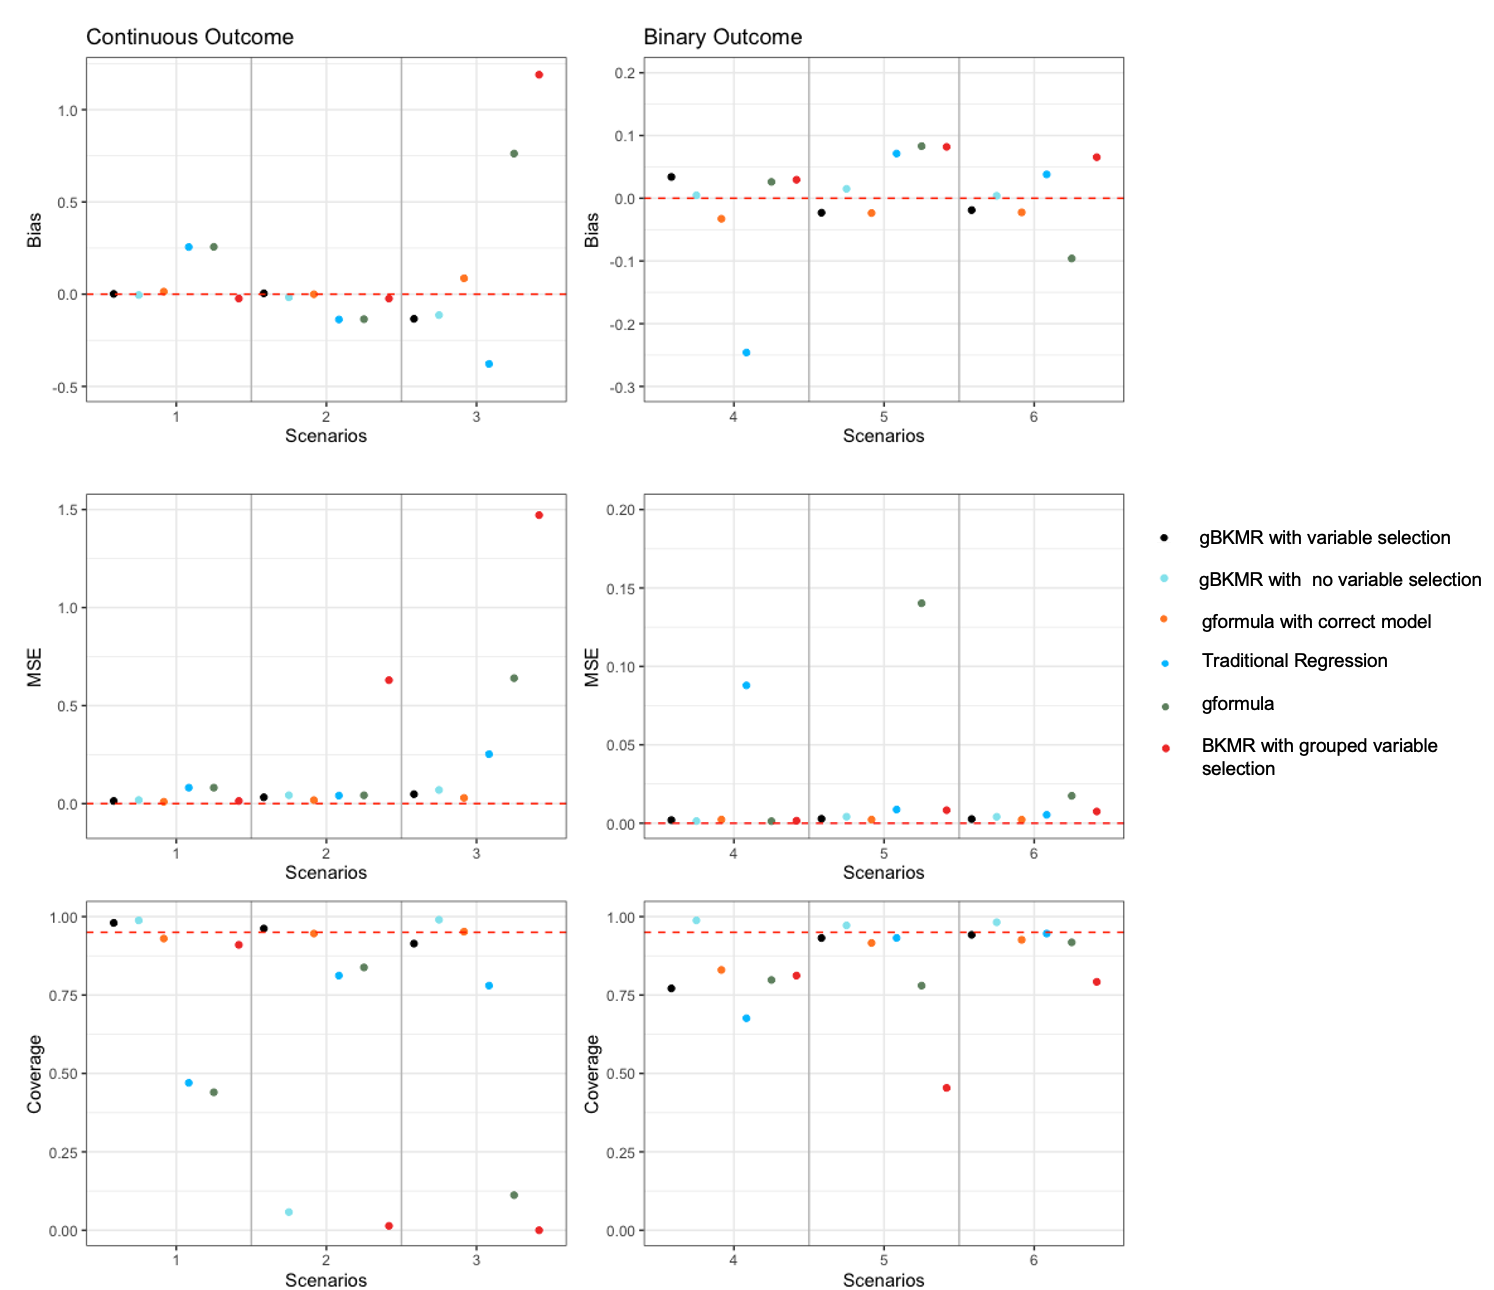
\includegraphics[width=0.95\textwidth]{figures/fig_simulation.png}
\caption{Bias, MSE, and coverage of the ATE estimates across the six simulation scenarios, comparing CausalBKMR (with and without variable selection) against the parametric g-formula, the parametric g-formula with correct model specification, traditional regression, and BKMR with grouped variable selection. Left column: continuous outcome (scenarios 1--3); right column: binary outcome (scenarios 4--6). Dashed red line indicates zero bias (top), zero MSE (middle), or nominal $95\%$ coverage (bottom).}
\label{fig:sim_results}
\end{figure}


\input{sections/results_application}

% ============================================================================
% Discussion (from Arce's gBKMR_Nature.docx; to be expanded by Linda + Arce)
% ============================================================================

\section*{Discussion}

Exposure to metal mixtures has been shown to increase the risk of several chronic diseases, including diabetes and cardiovascular disease. In this study, we present a novel method, g-BKMR, to estimate the joint effect of multiple time-varying exposures over time while adjusting for time-varying confounders. Our approach allows the estimation of joint effects and interactions of time-varying environmental exposures, which is critical for understanding the complex relationships between exposures and health outcomes. Moreover, our method accounts for time-varying confounding, and could also be extended to help mitigate potential biases that may arise from unmeasured confounding factors.

The g-formula used in our method allows for complex relationships between the elements of the mixture and the confounders through the joint kernel specification in the outcome model. Beyond environmental health, our proposed method can be applied to a wide range of data with high-dimensional time-varying correlated exposures when causal interpretation is desired.

Applying g-BKMR to the Strong Heart Study, we found a harmful effect of co-exposure to six urinary metals on fasting blood glucose. Zinc was the dominant contributor to the joint mixture signal across all three visits, while selenium at Visit~1 showed a positive association that was robust to excluding participants with baseline diabetes---consistent with evidence from the Selenium and Vitamin E Cancer Prevention Trial (SELECT) that selenium supplementation elevates diabetes risk.\cite{select_trial} Cadmium at Visit~1 showed an inverse association that remained after adjustment for baseline pack-years, suggesting the pattern is not solely explained by smoking intensity. These findings highlight the importance of addressing exposure to metal mixtures in the prevention of diabetes and cardiovascular disease. Our simulation study also showed that g-BKMR outperforms other existing methods for the evaluation of environmental mixtures with repeated measures.

In conclusion, the g-BKMR method provides a powerful and flexible approach to estimate the joint effects of time-varying exposures, while accounting for time-varying confounders, and can be applied to a wide range of data. The findings from our application of g-BKMR to the Strong Heart Study underscore the importance of addressing exposure to metal mixtures in the prevention of chronic diseases. g-BKMR enables a better understanding of the complex relationship between environmental mixtures and health outcomes, paving the way for more effective public health policies and interventions.


% ============================================================================
% DECLARATIONS
% ============================================================================
\section*{Declarations}

\subsection*{Funding}
% TODO: Grant numbers from each author's institution.

\subsection*{Availability of data and materials}
The CausalBKMR R package is publicly available on GitHub at \url{https://github.com/zc2326/causalbkmr}. Strong Heart Study data are available from the SHS Coordinating Center upon request and after approval by the participating American Indian tribes.

\subsection*{Code availability}
All code used in this manuscript is included in the package or its supplement.

\subsection*{Ethics approval and consent to participate}
The Strong Heart Study was approved by the Indian Health Service Institutional Review Board, the institutional review boards of the participating American Indian tribes, and the institutional review boards of the participating institutions. All participants provided written informed consent.

\subsection*{Author contributions}
% TODO: detailed contributions (ZC developed the original method; AD-R and YL implemented the software; YL conducted the SHS application; etc.)

\subsection*{Competing interests}
The authors declare no competing interests.

\subsection*{Acknowledgements}
% TODO: tribes, study staff, funding bodies.

% ============================================================================
% REFERENCES
% ============================================================================
\bibliography{references}

% ============================================================================
% SUPPLEMENTARY MATERIAL
% ============================================================================
\clearpage
\appendix
\section*{Supplementary Material}

\renewcommand{\thefigure}{S\arabic{figure}}
\setcounter{figure}{0}

% ============================================================================
% Supplementary Figures
% Shared between Supplementary.tex (standalone) and main_nature.tex (full paper)
% ============================================================================

% ---- S1: Per-metal dose-response (full) ----
\begin{figure}[h]
\centering
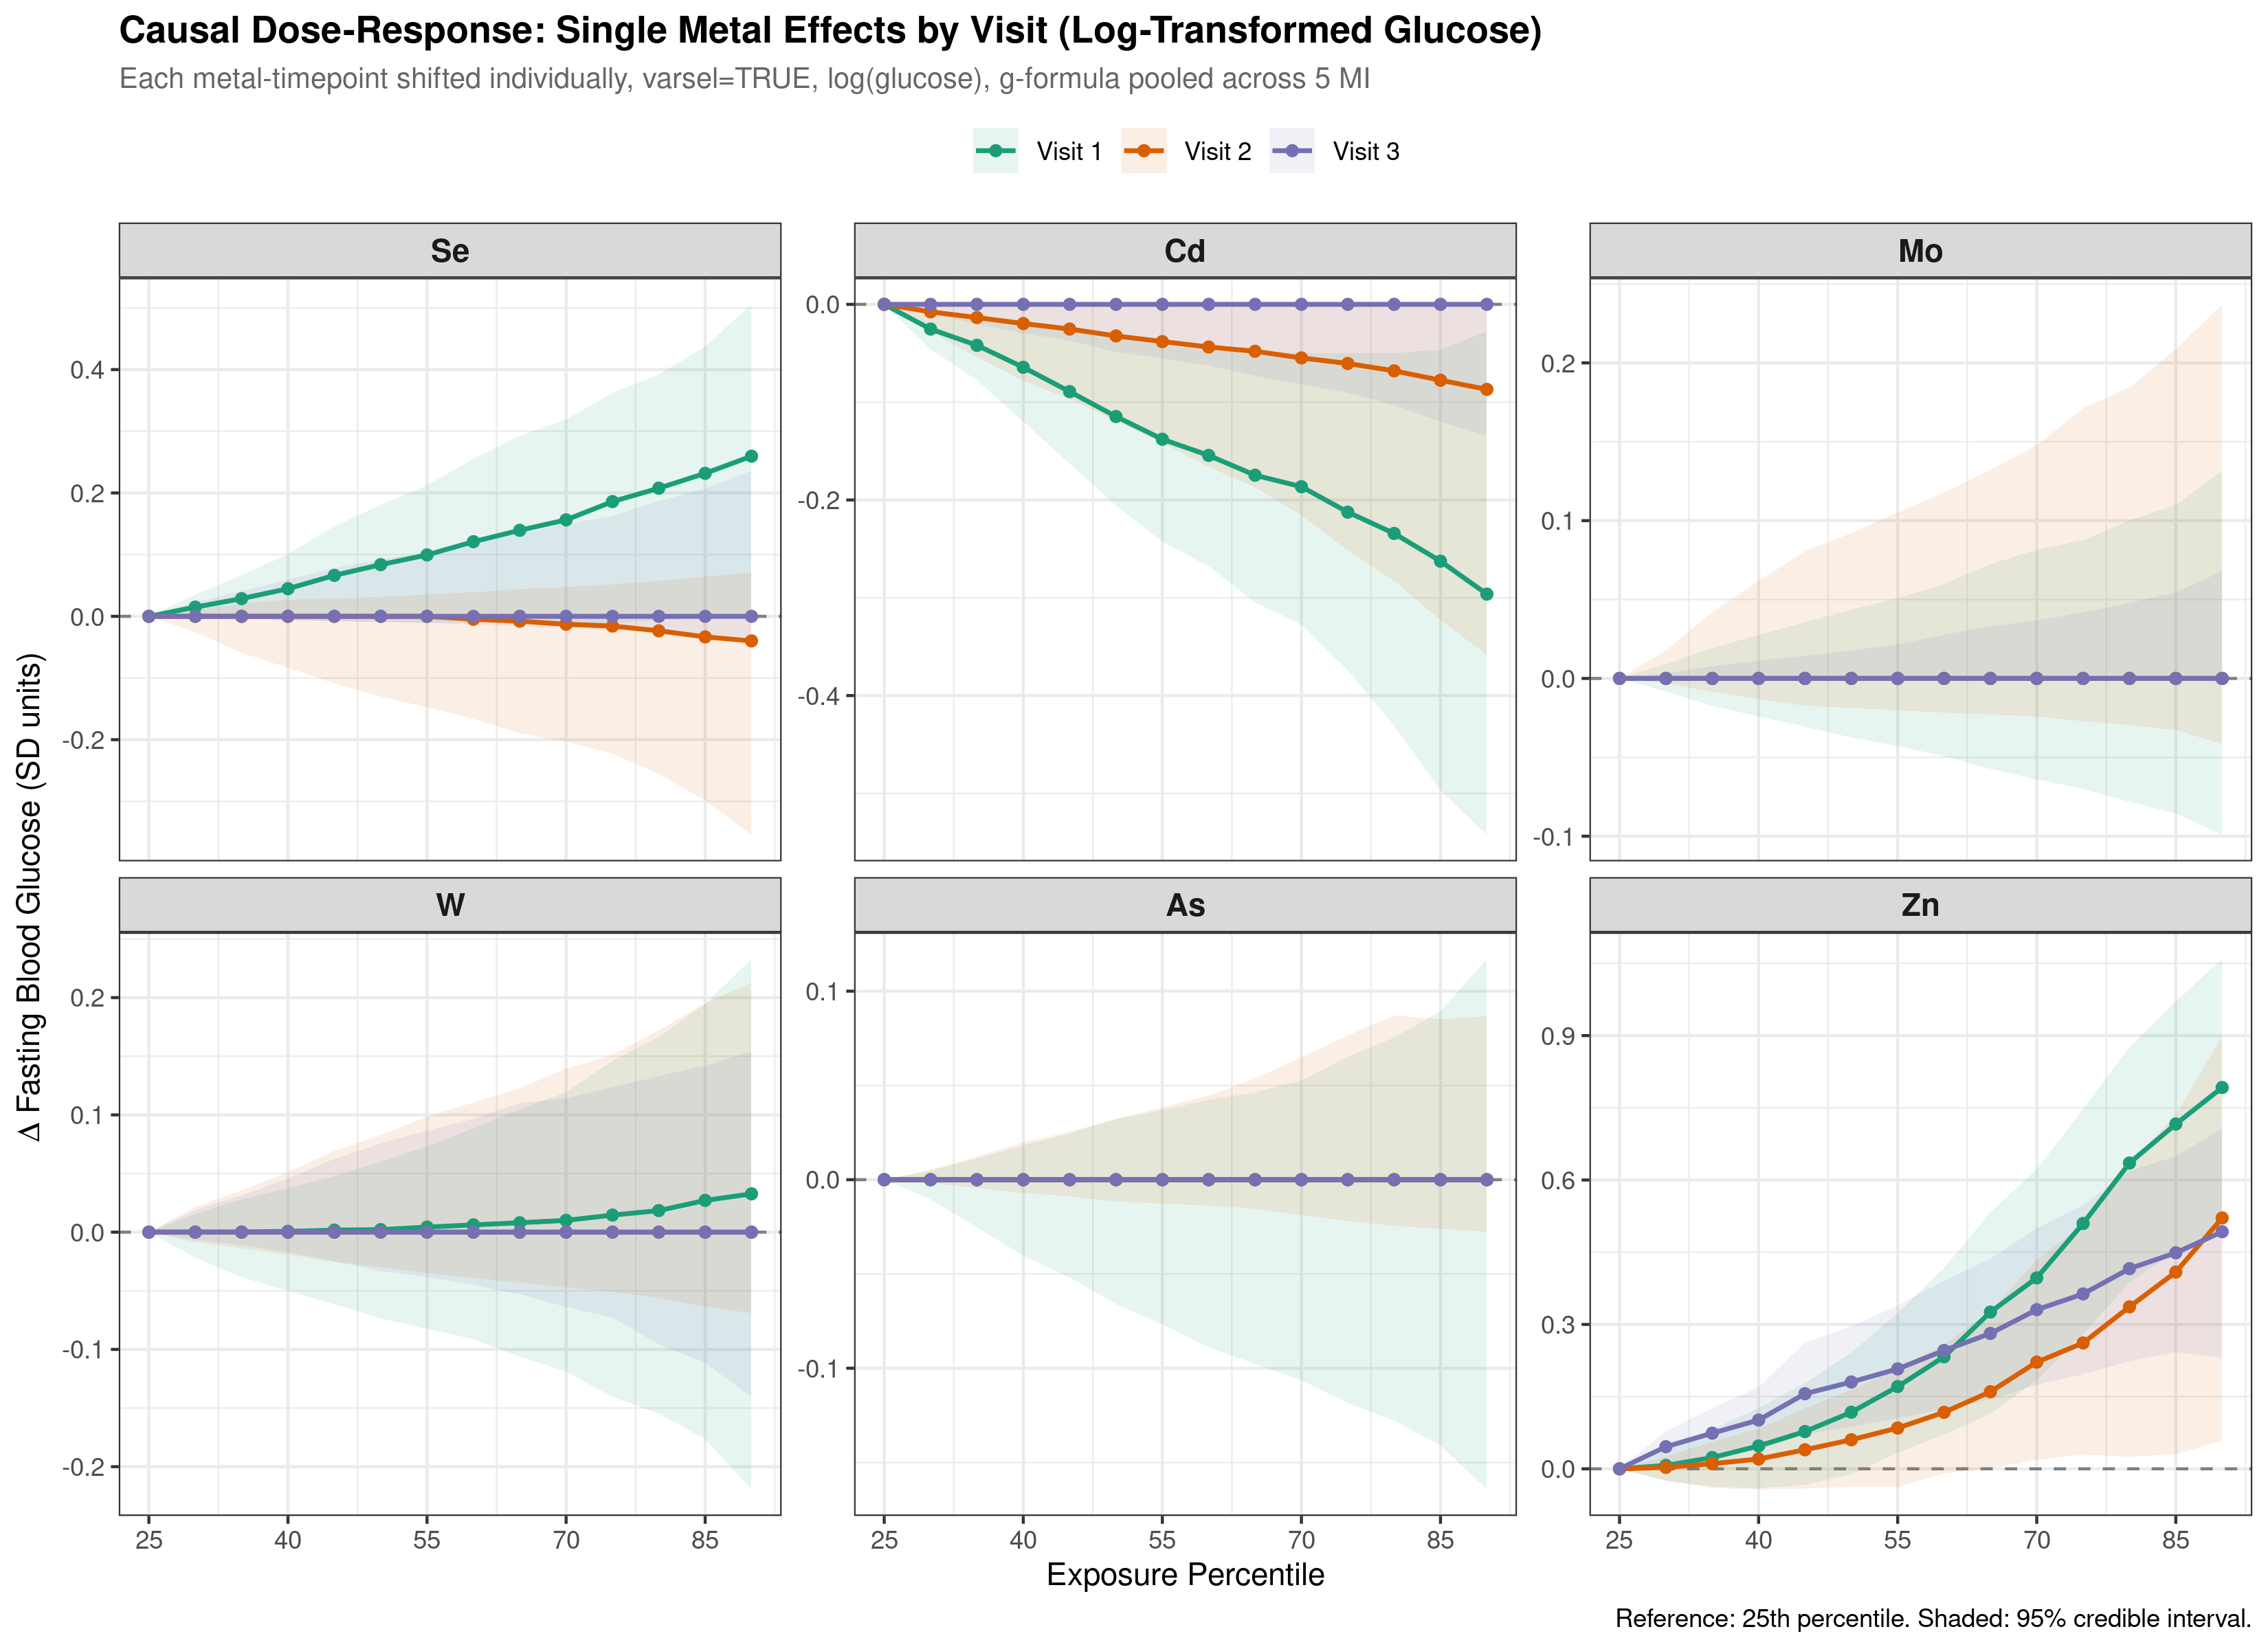
\includegraphics[width=0.85\textwidth]{figures/fig_permetal_full.png}
\caption{Per-metal dose-response curves (full sample, $n = 679$). Each panel: one metal shifted across percentiles, remaining exposures at the 50th percentile. Lines distinguish the three visits.}
\end{figure}

% ---- S2: Forest no-DM ----
\begin{figure}[h]
\centering
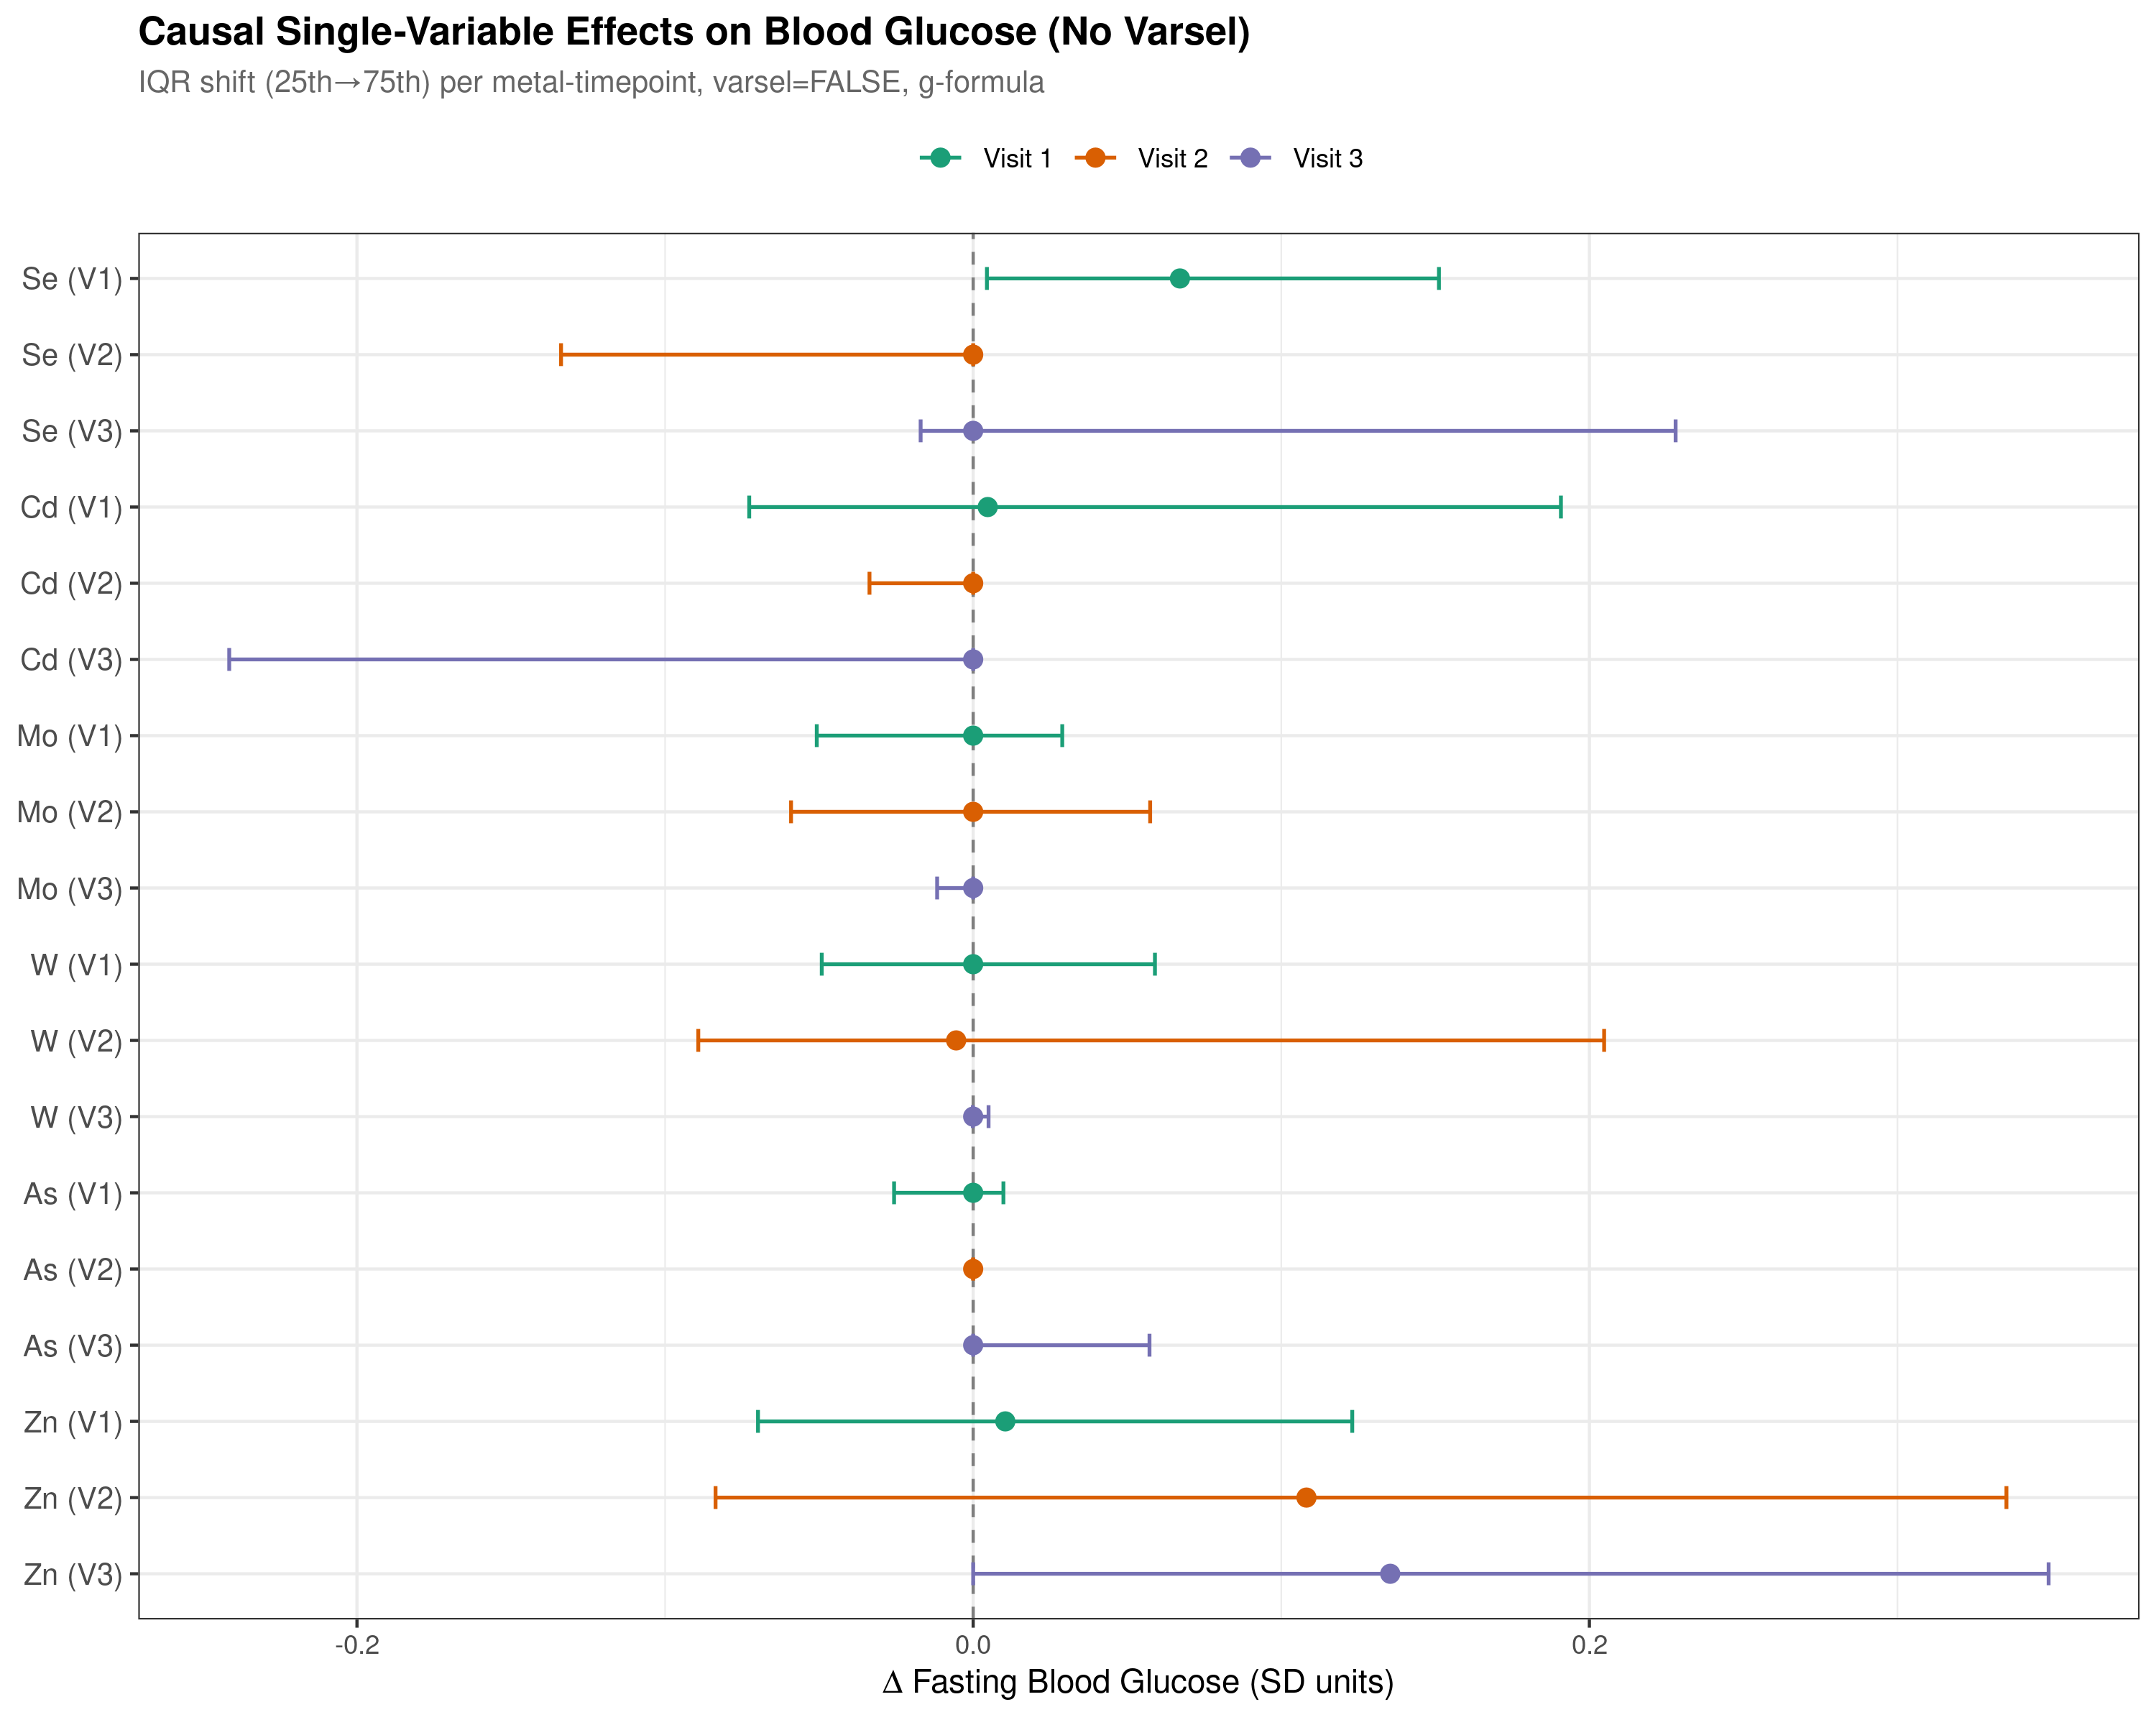
\includegraphics[width=0.85\textwidth]{figures/fig_forest_nodm.png}
\caption{Single-variable causal effects, excluding baseline diabetes ($n = 414$).}
\end{figure}

% ---- S3: Per-metal dose-response (no-DM) ----
\begin{figure}[h]
\centering
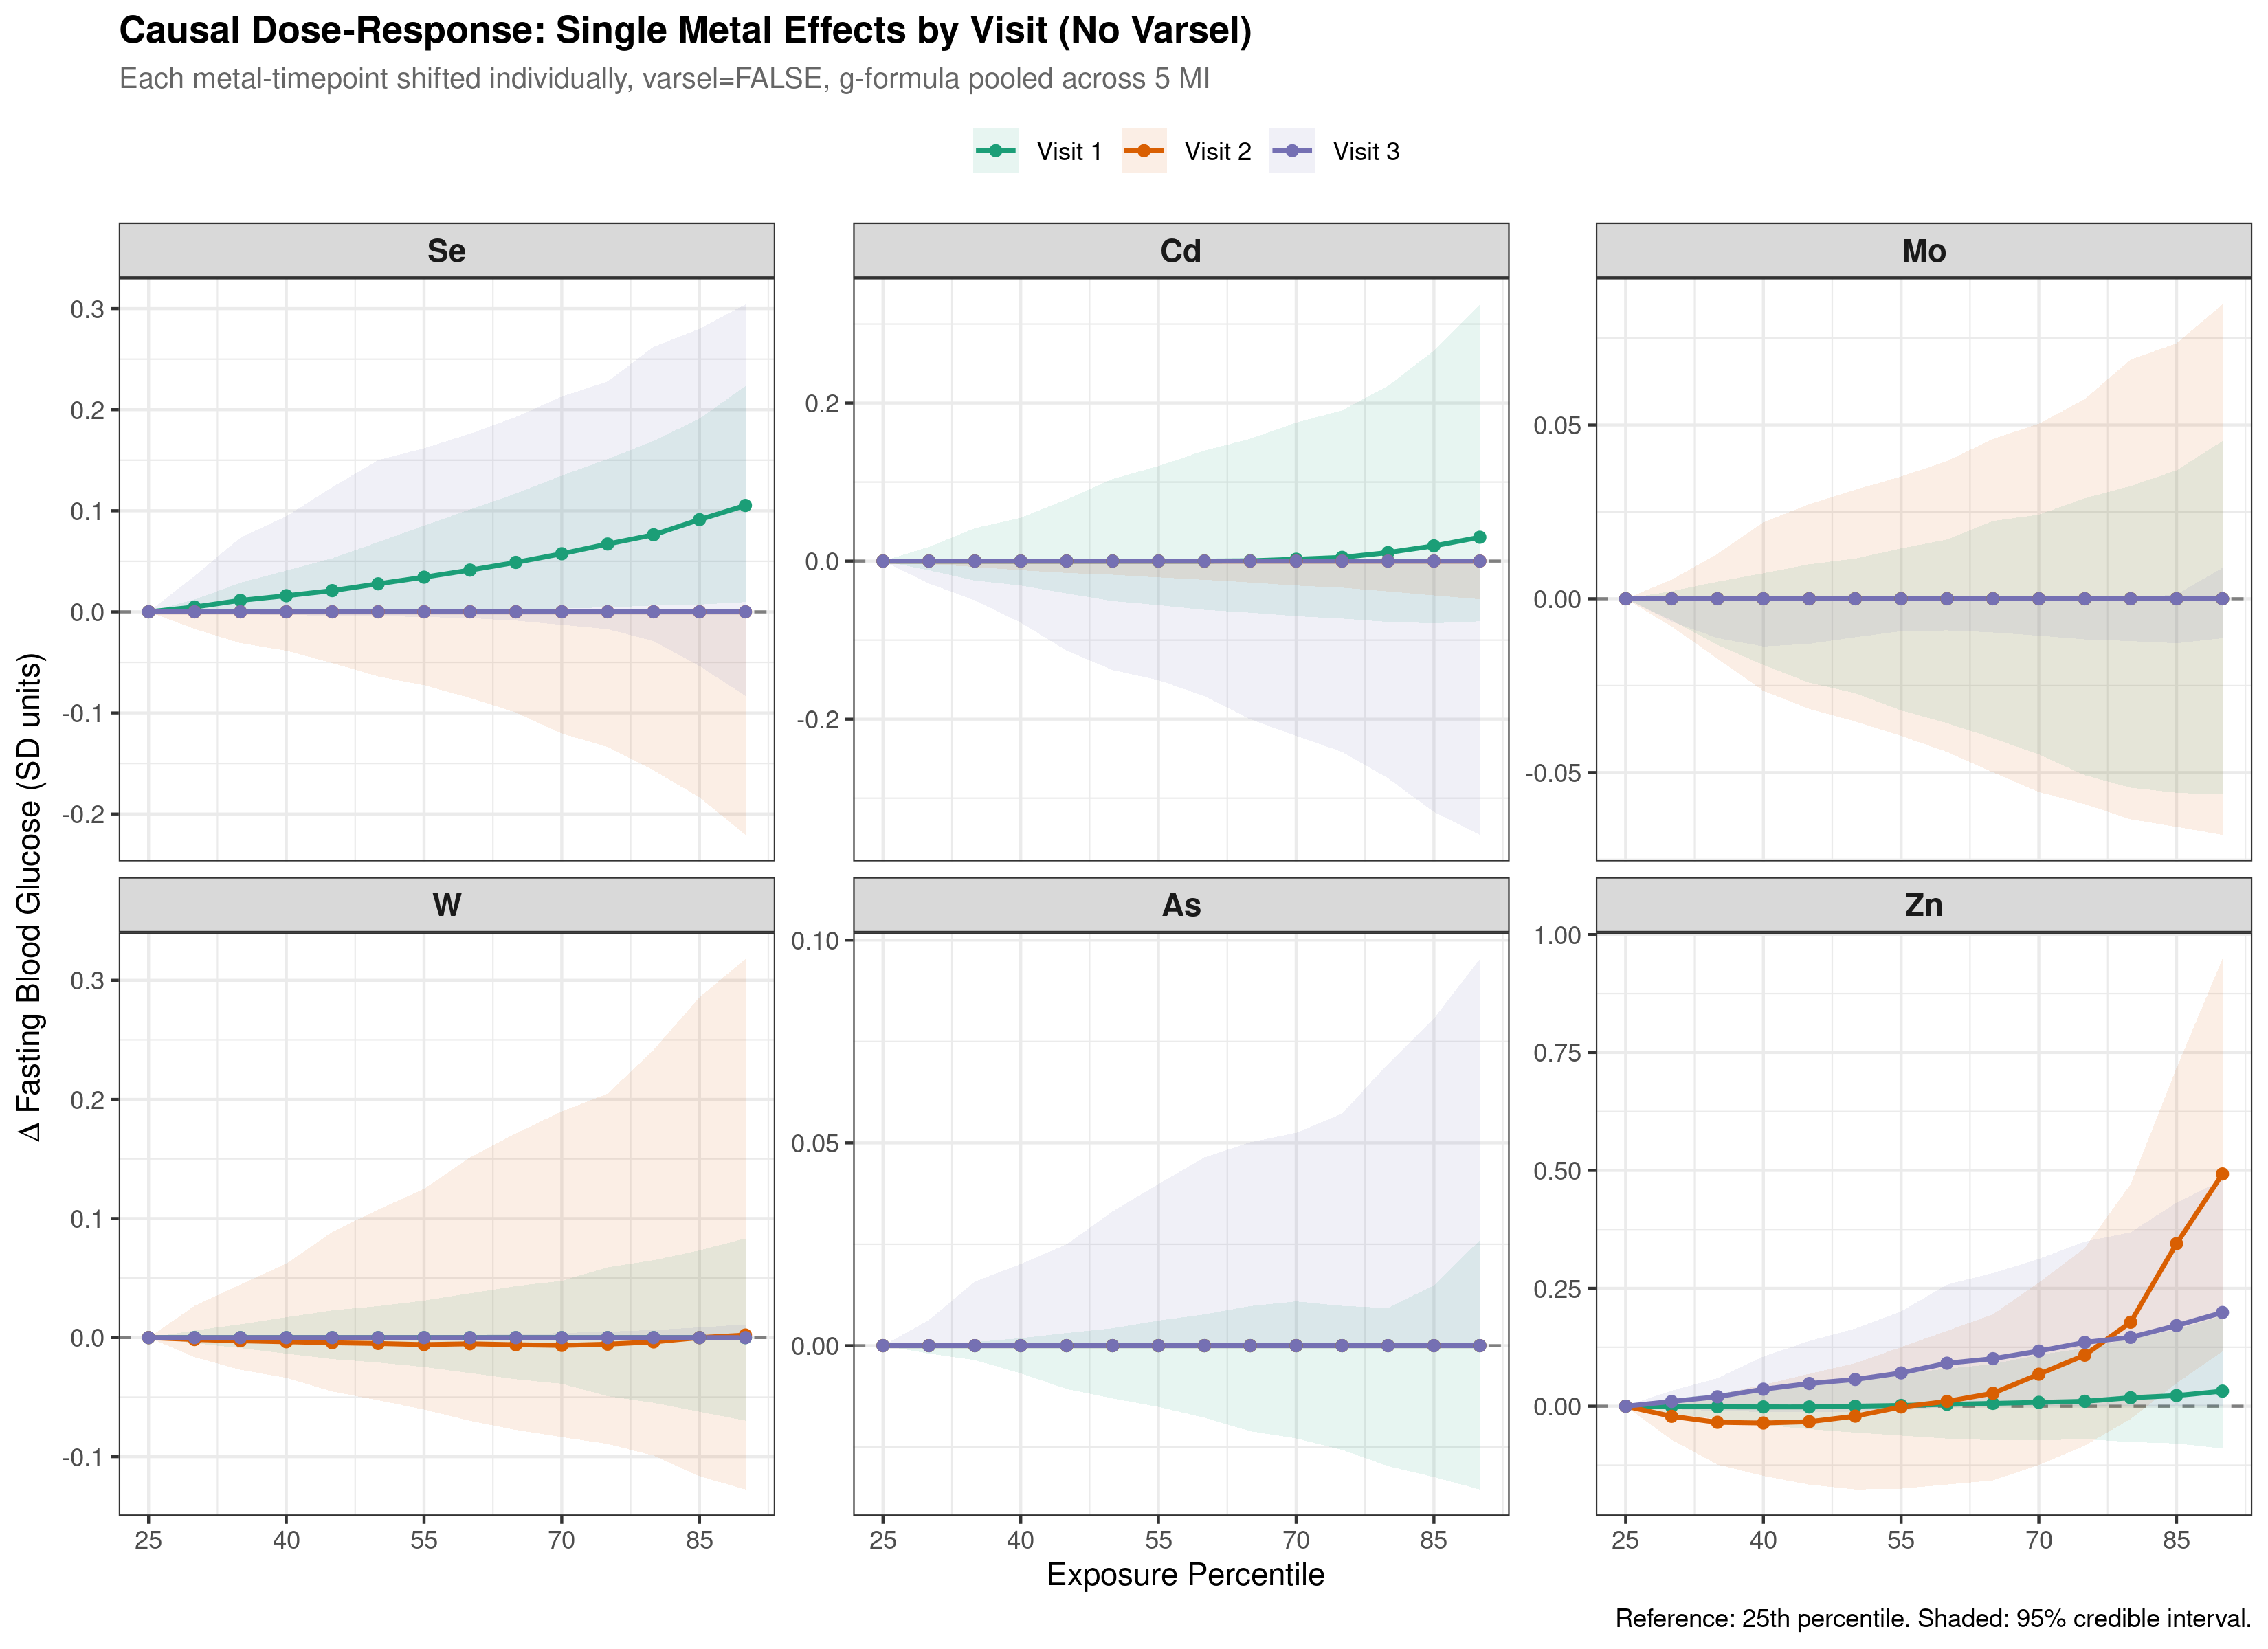
\includegraphics[width=0.85\textwidth]{figures/fig_permetal_nodm.png}
\caption{Per-metal dose-response curves, excluding baseline diabetes ($n = 414$).}
\end{figure}

% ---- S4: Dose-response pack-years ----
\begin{figure}[h]
\centering
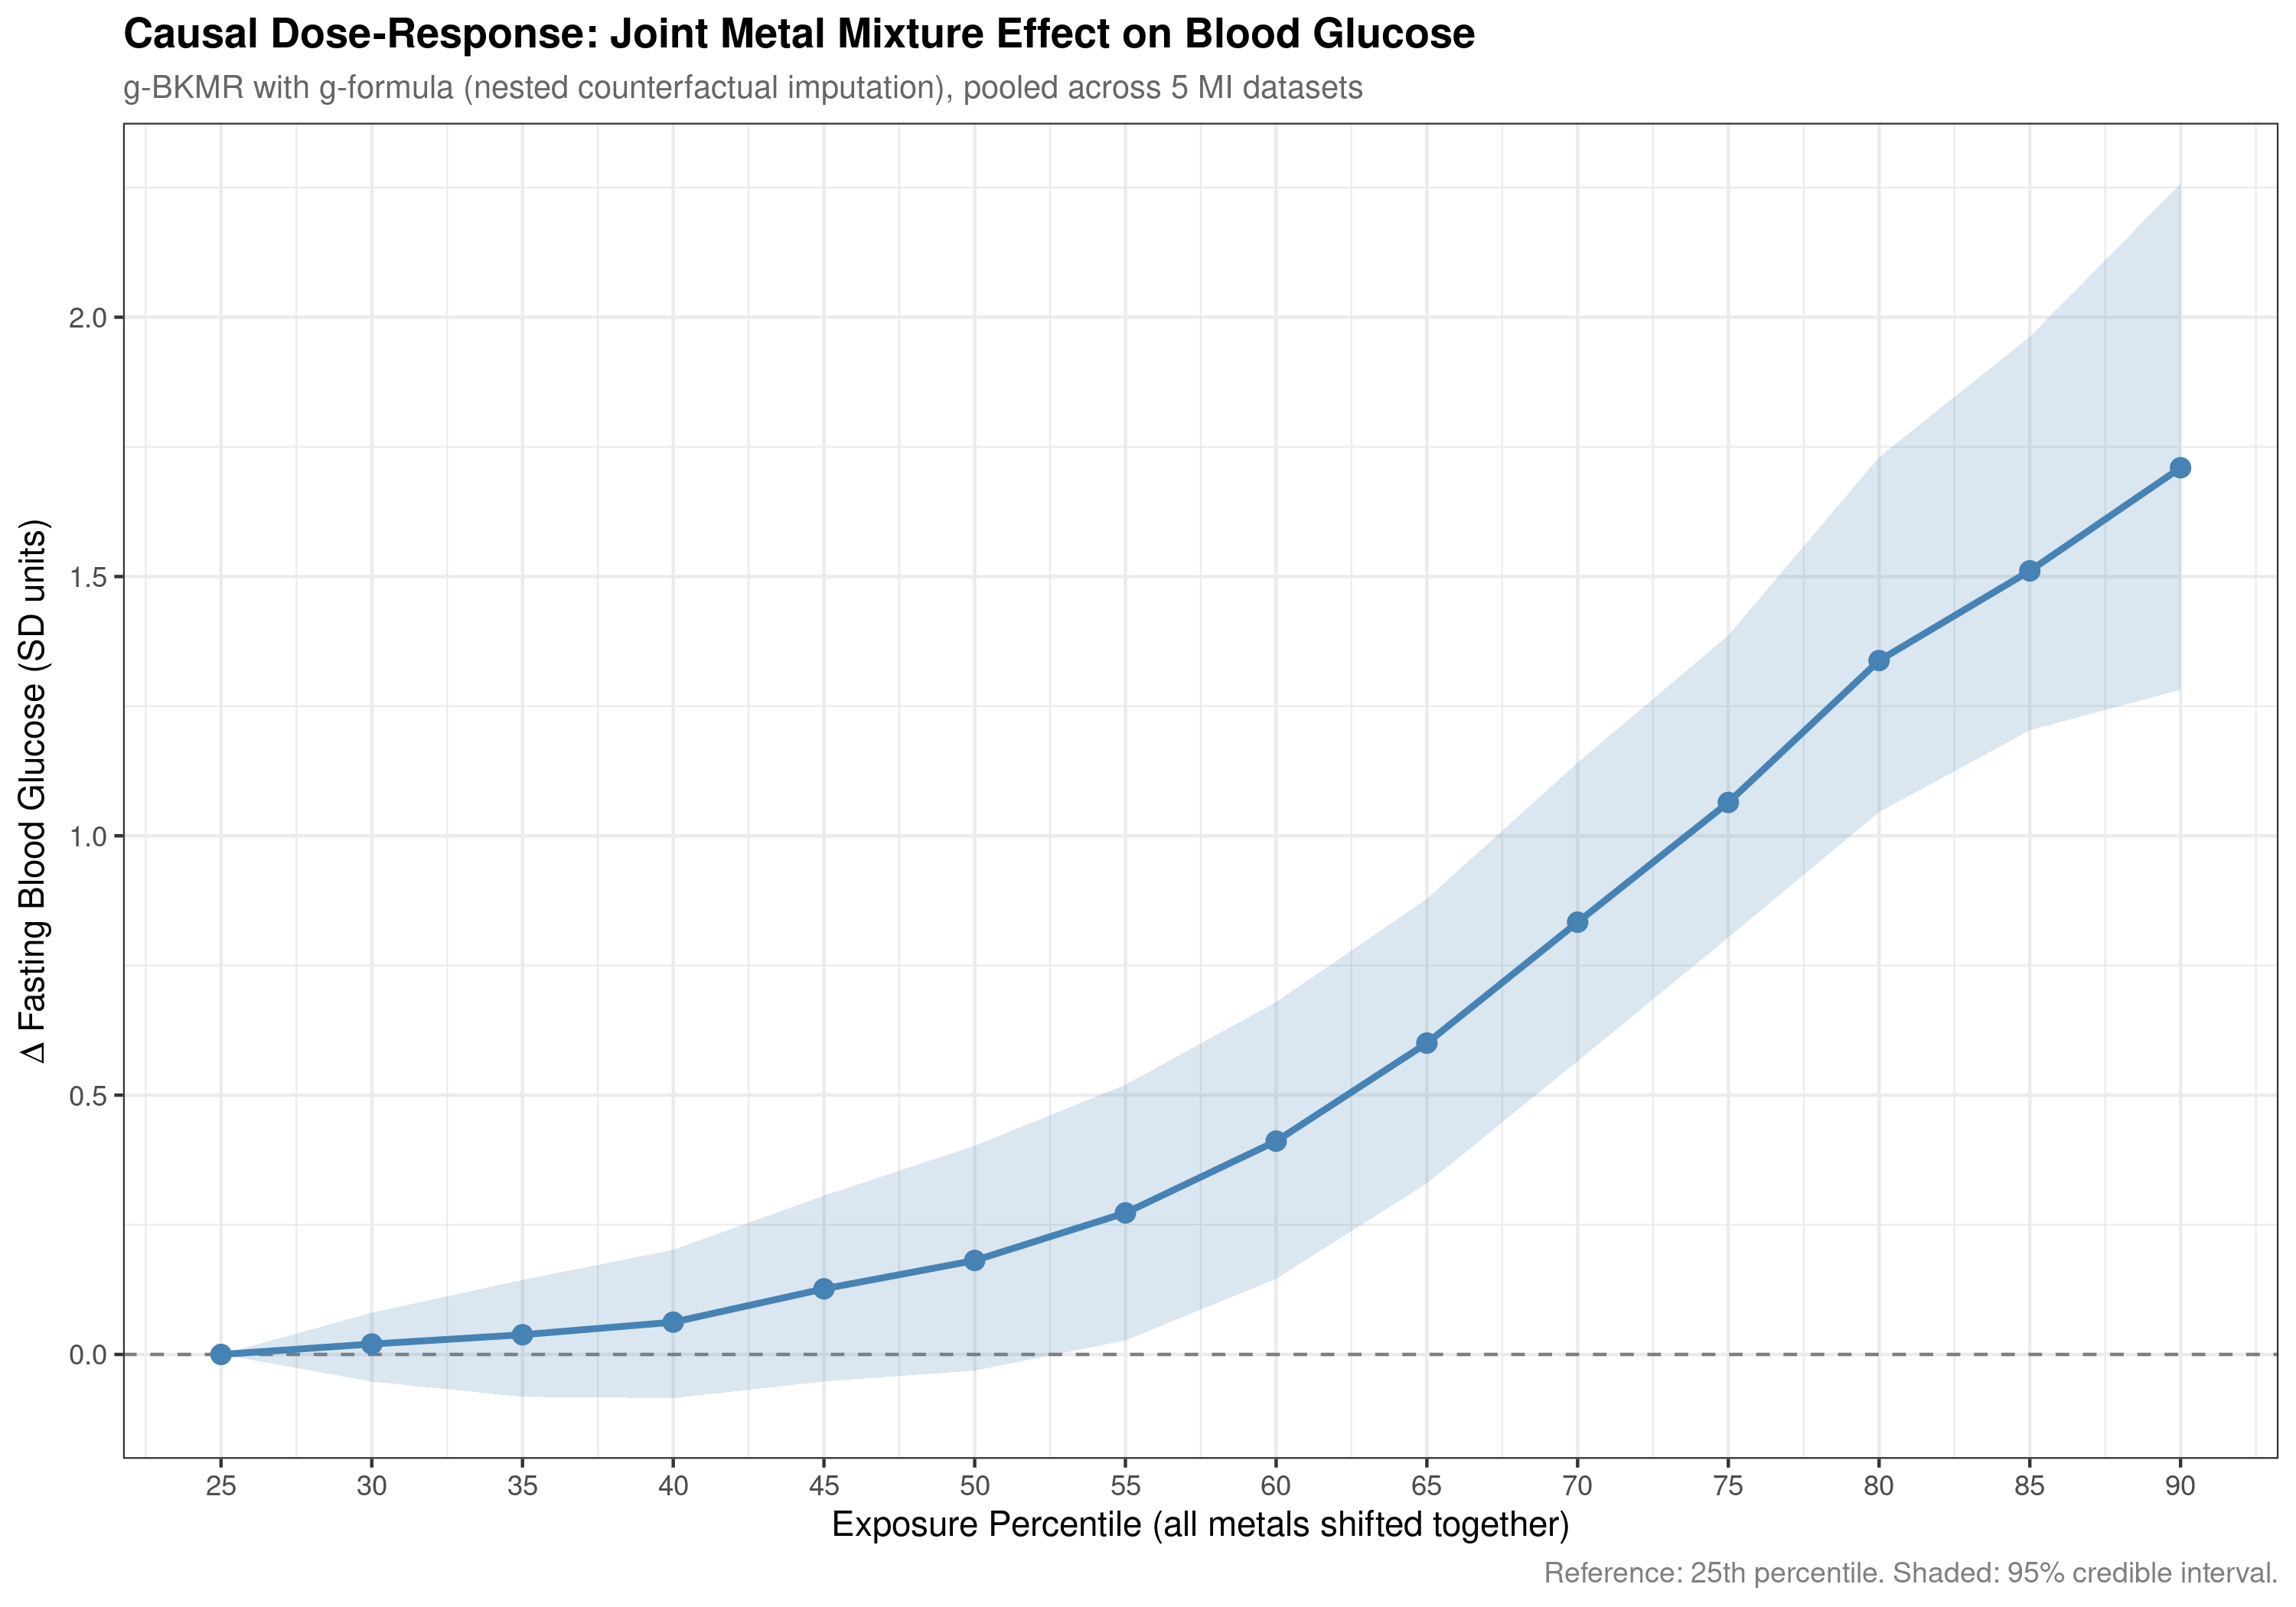
\includegraphics[width=0.85\textwidth]{figures/fig_dr_packyears.png}
\caption{Sensitivity: joint dose-response after additionally adjusting for baseline pack-years ($n = 679$).}
\end{figure}

% ---- S5: Forest pack-years ----
\begin{figure}[h]
\centering
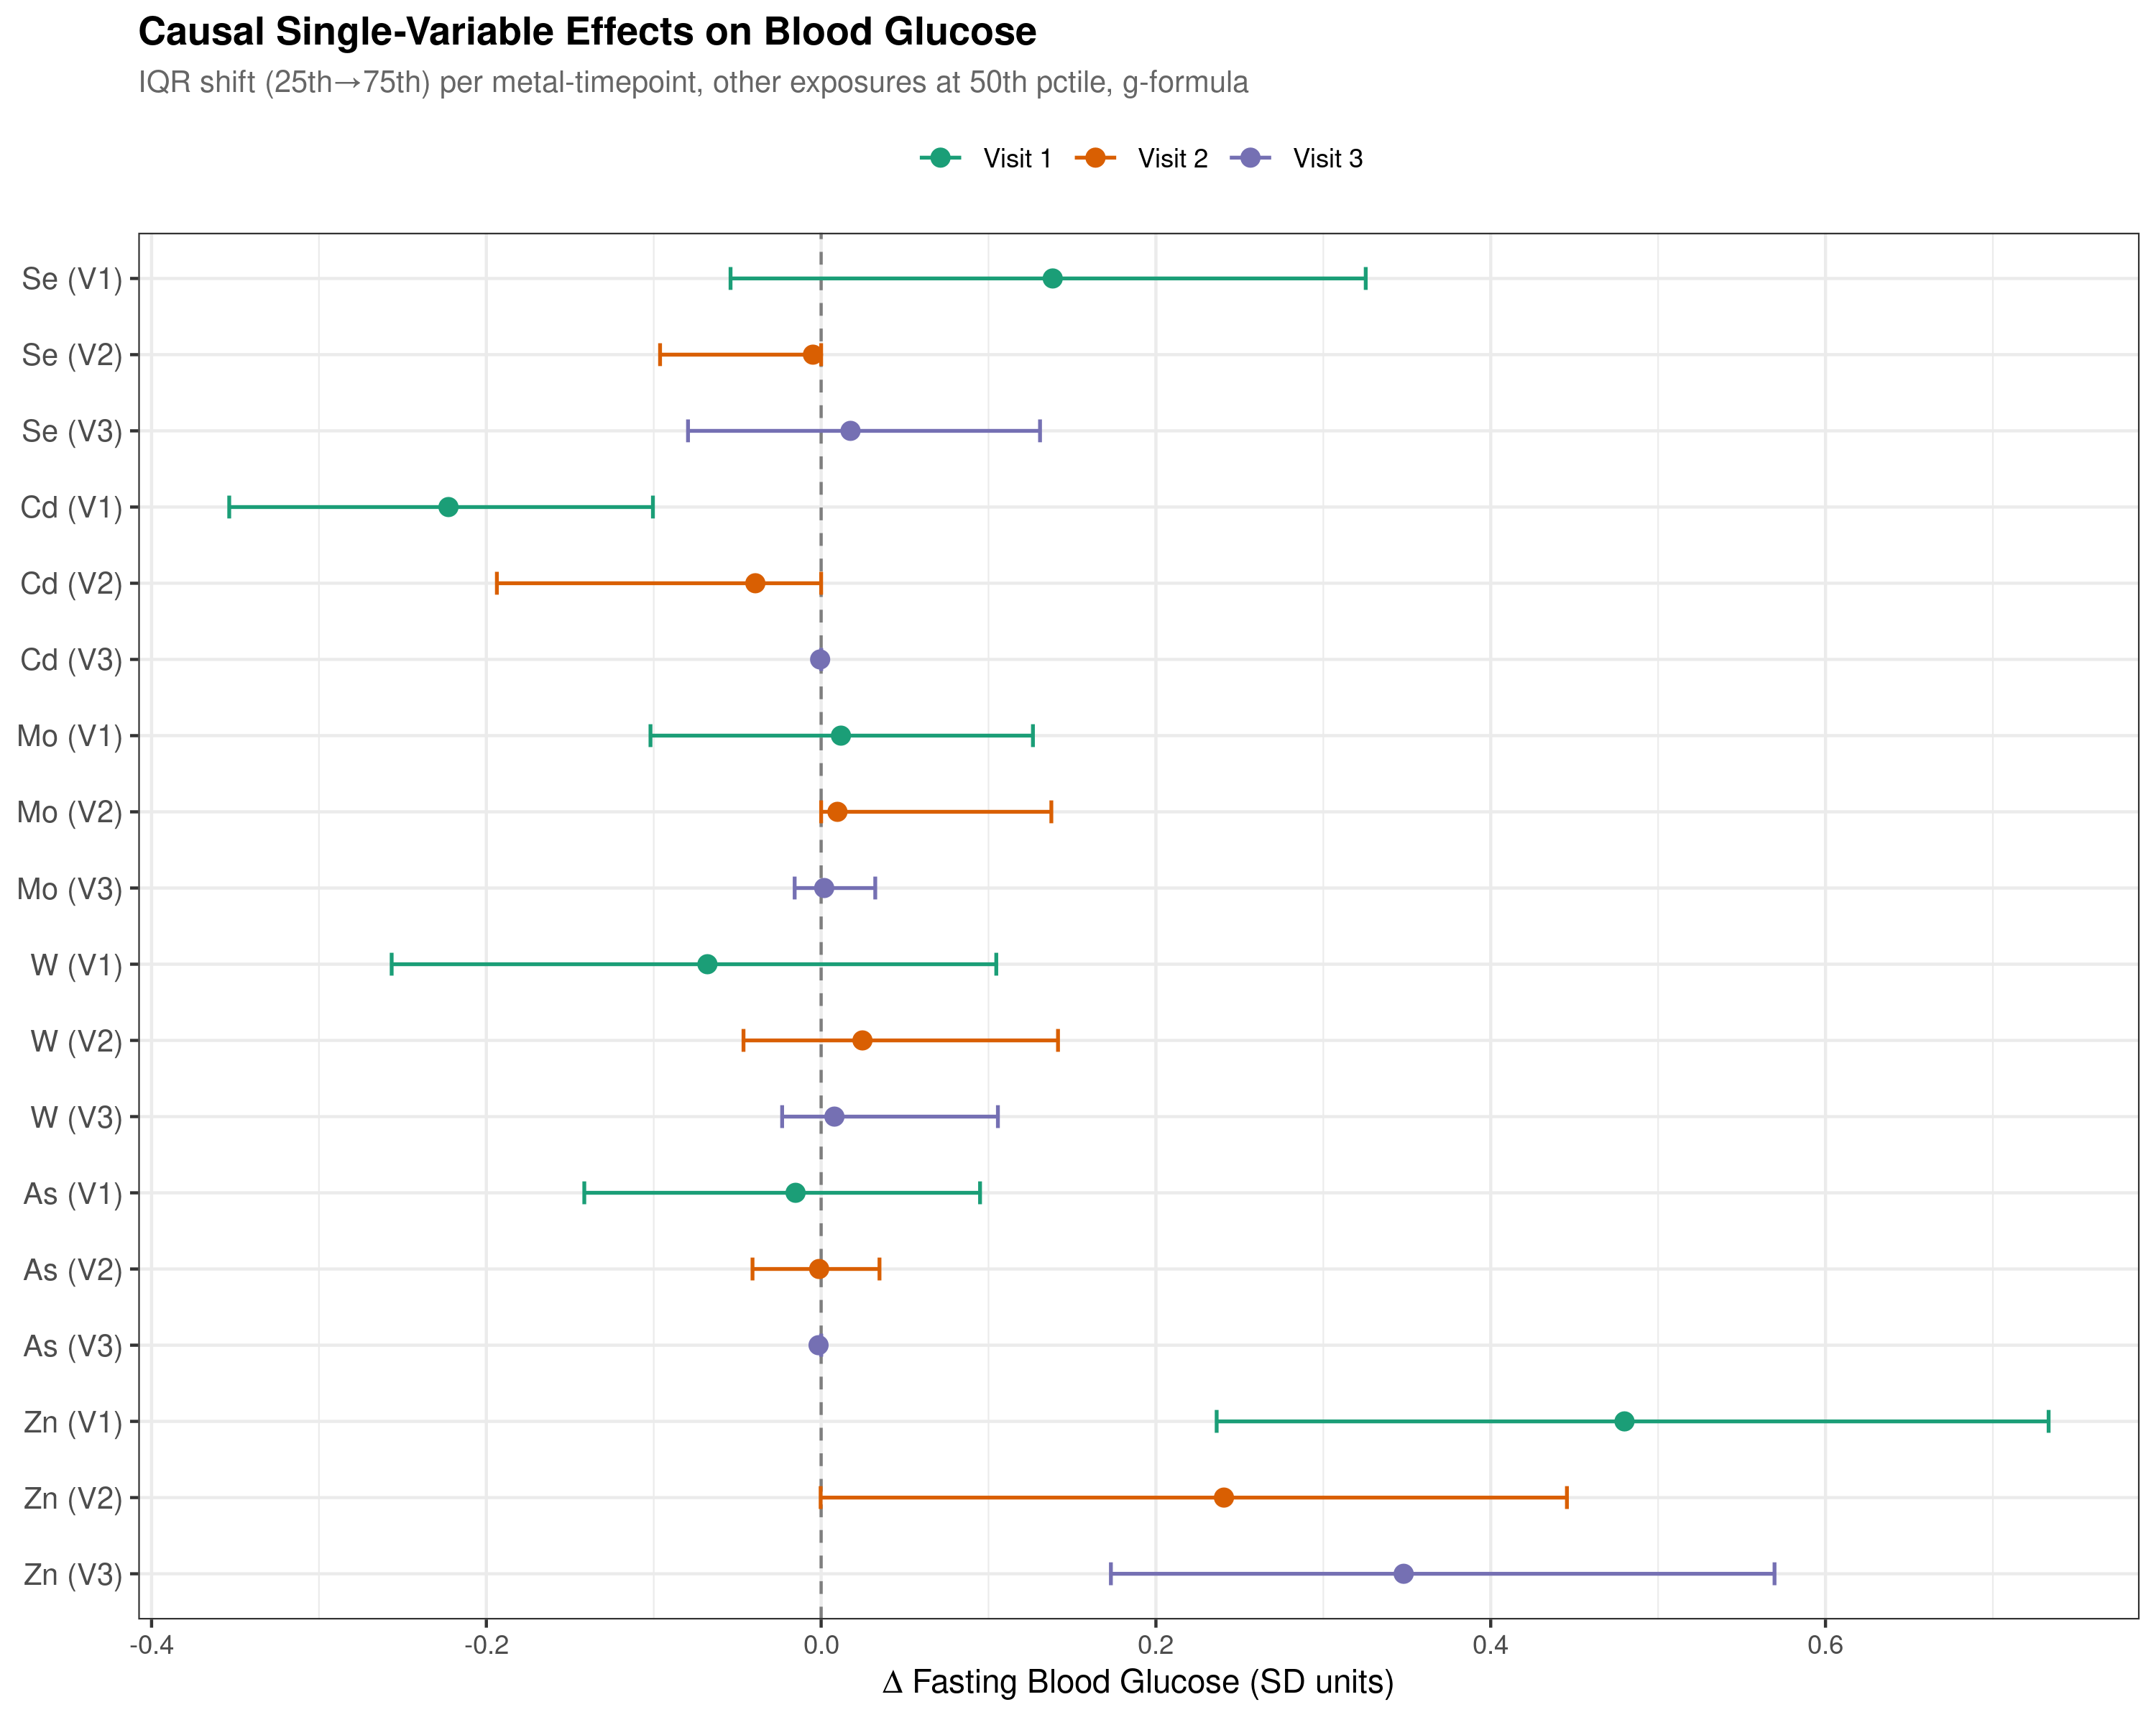
\includegraphics[width=0.85\textwidth]{figures/fig_forest_packyears.png}
\caption{Sensitivity: single-variable causal effects after additionally adjusting for baseline pack-years ($n = 679$).}
\end{figure}

% ---- S6: Per-metal dose-response pack-years ----
\begin{figure}[h]
\centering
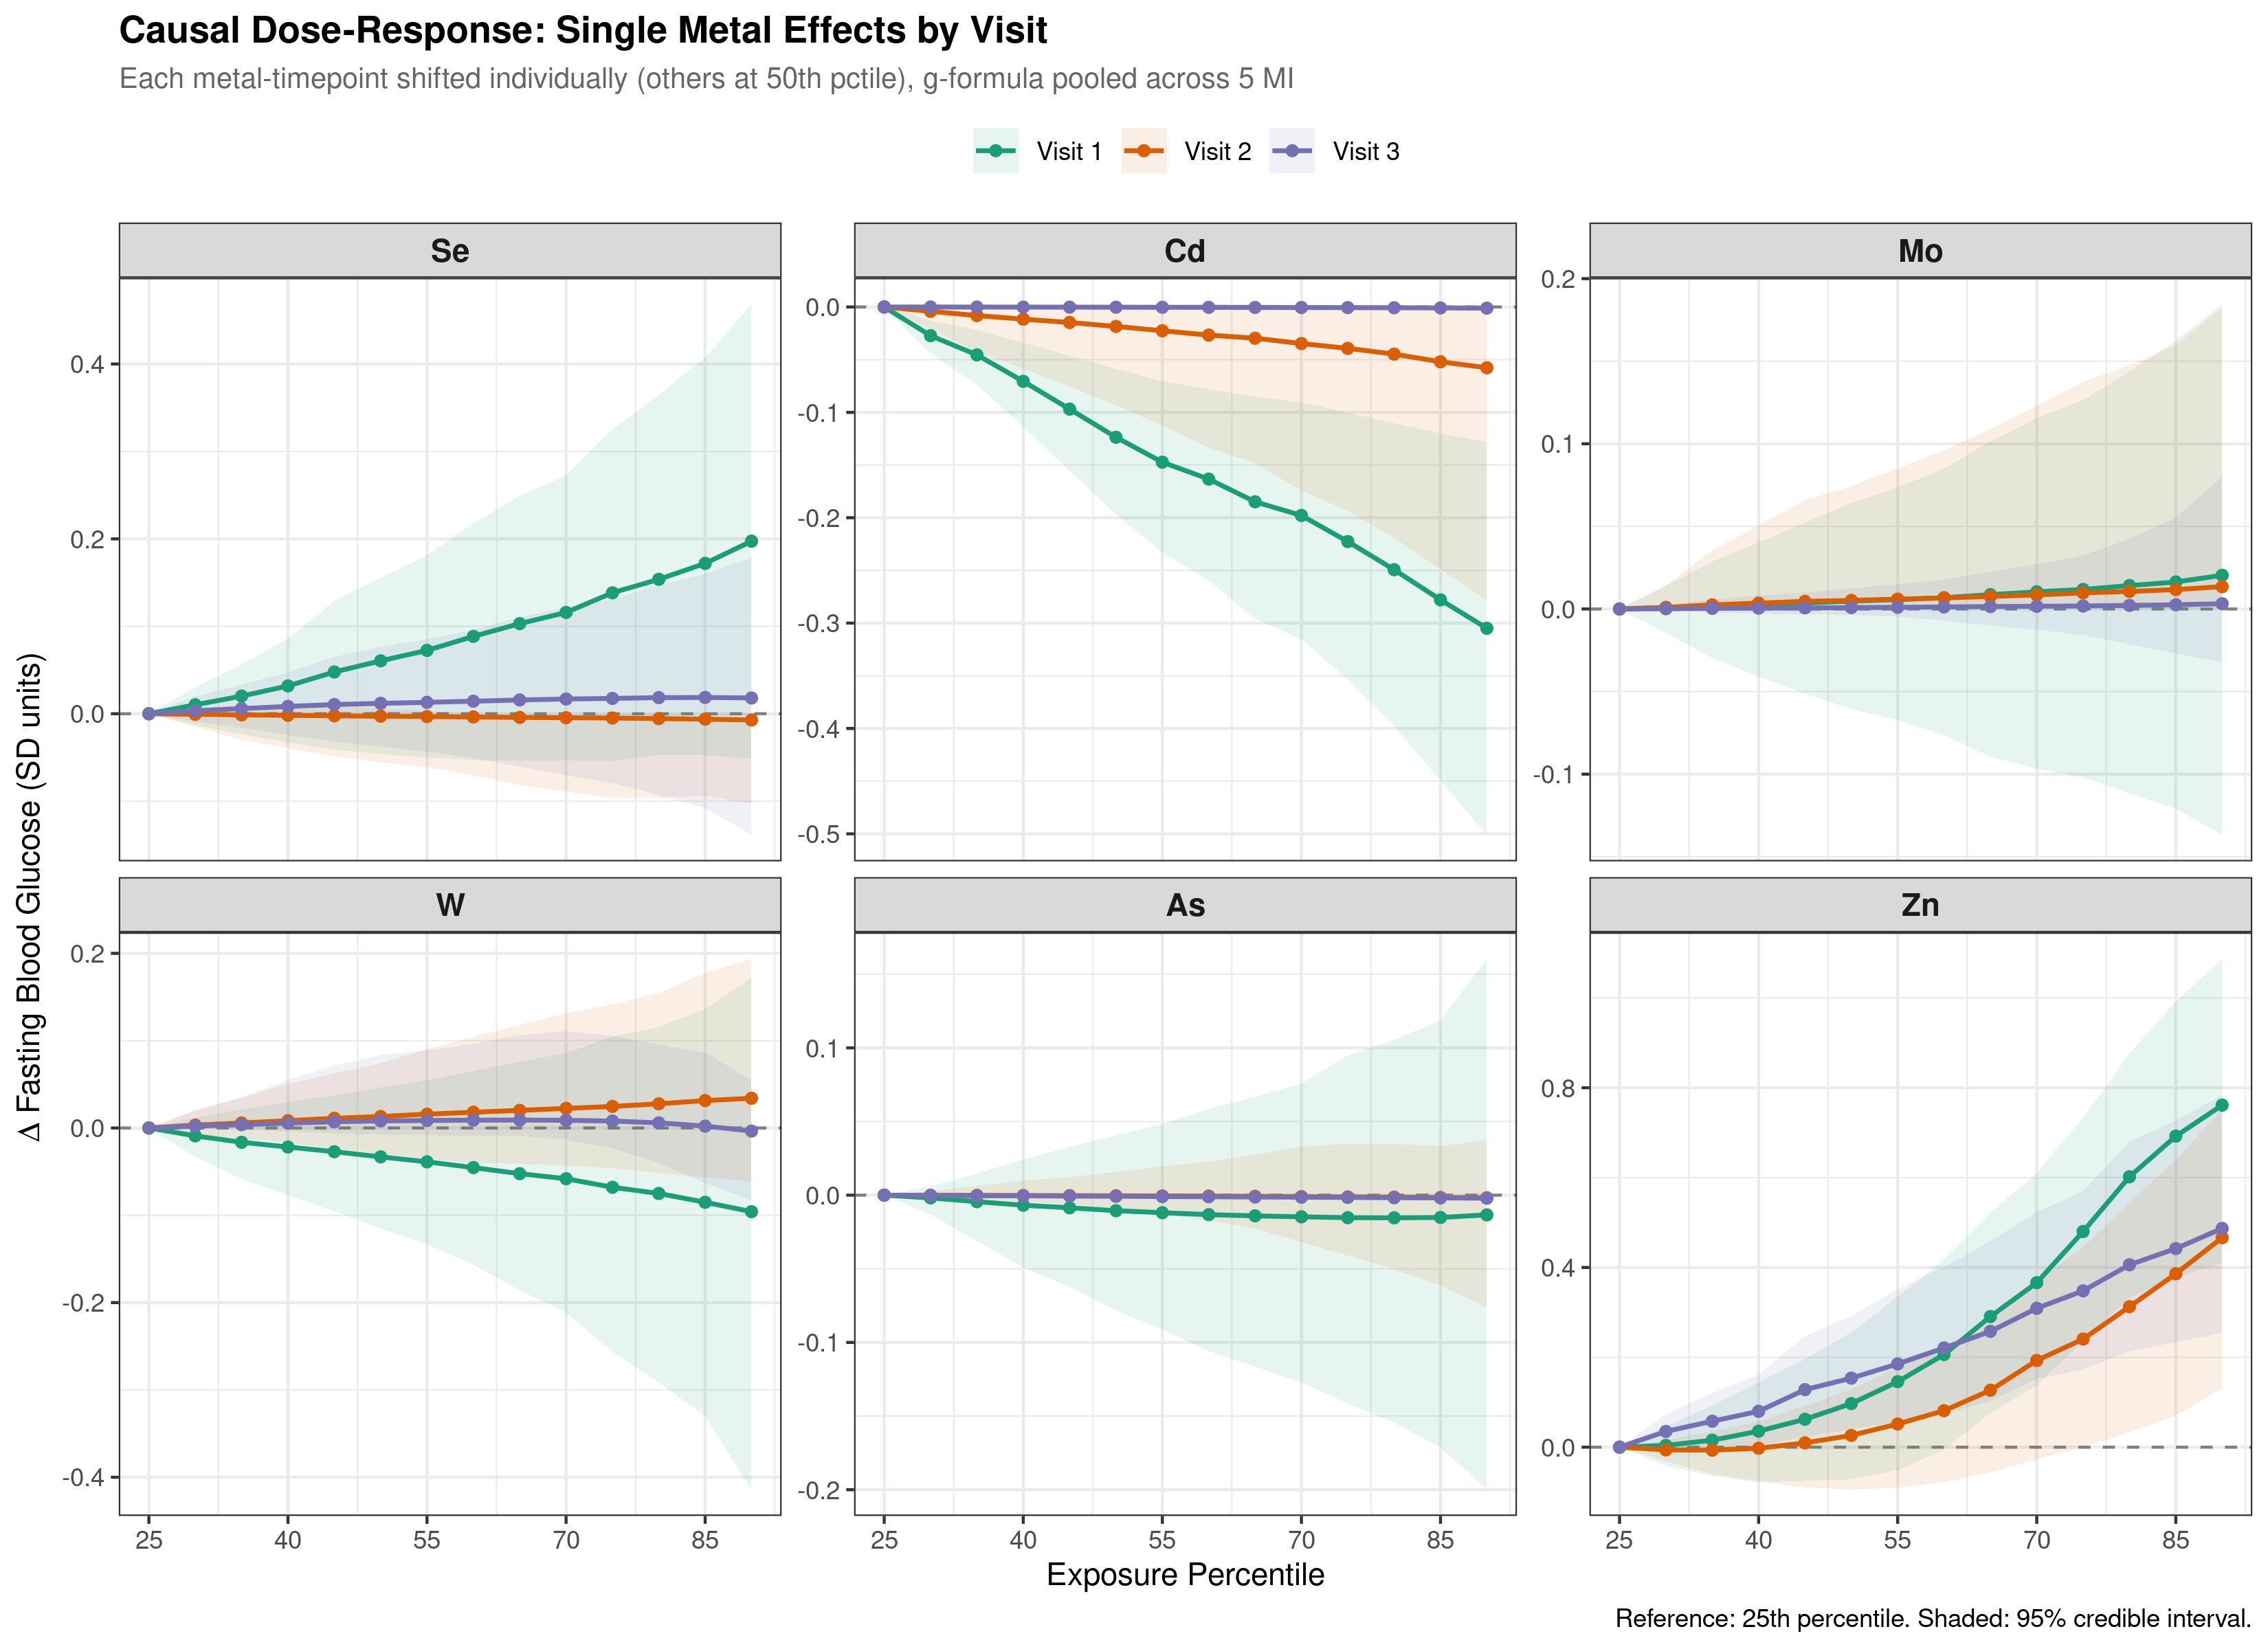
\includegraphics[width=0.85\textwidth]{figures/fig_permetal_packyears.png}
\caption{Sensitivity: per-metal dose-response curves after additionally adjusting for baseline pack-years ($n = 679$).}
\end{figure}

% ---- S7: MCMC trace plots ----
\begin{figure}[h]
\centering
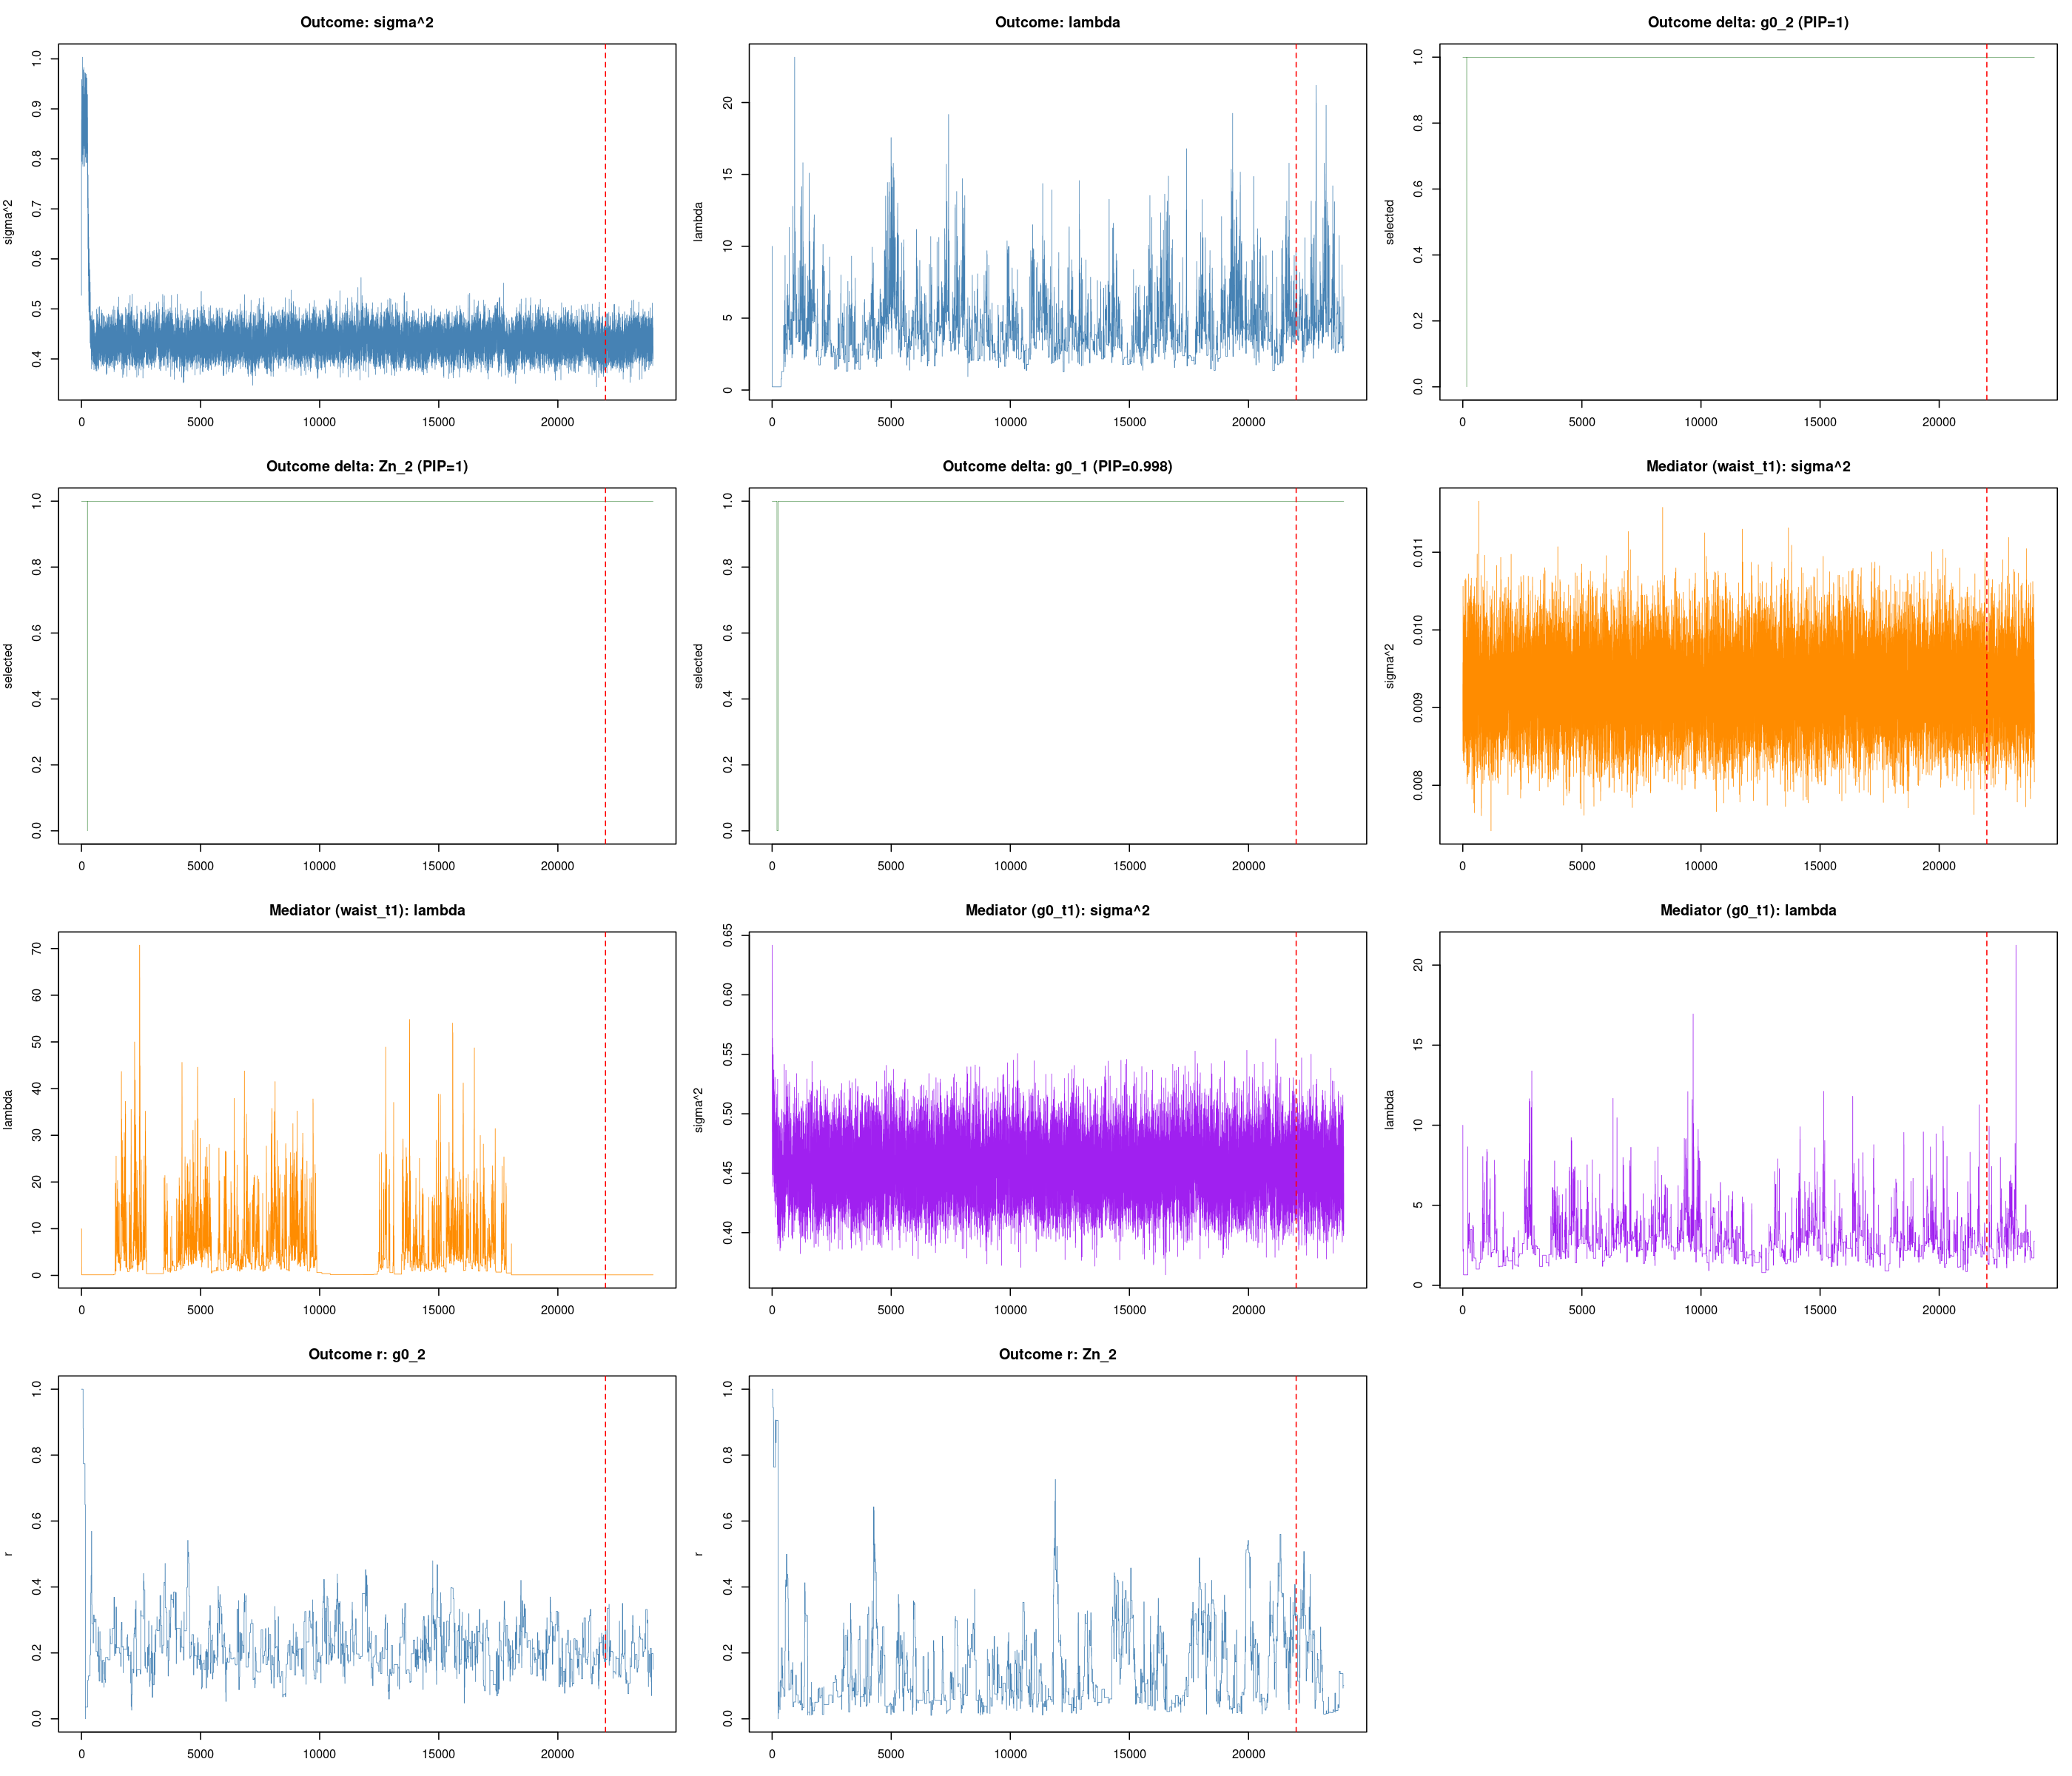
\includegraphics[width=0.9\textwidth]{figures/fig_traceplots.png}
\caption{MCMC trace plots for representative BKMR models in the main analysis. Chains showed good mixing, rapid transit between regions of the posterior, and no drift, indicating appropriate convergence for the retained posterior window (iterations $22{,}000$--$24{,}000$).}
\end{figure}


\end{document}
